% !TEX TS-program = pdflatex
% !TEX encoding = UTF-8 Unicode

% This is a simple template for a LaTeX document using the "article" class.
% See "book", "report", "letter" for other types of document.

\documentclass[11pt]{article} % use larger type; default would be 10pt

\usepackage[utf8]{inputenc} % set input encoding (not needed with XeLaTeX)

%%% Examples of Article customizations
% These packages are optional, depending whether you want the features they provide.
% See the LaTeX Companion or other references for full information.

%%% PAGE DIMENSIONS
\usepackage{geometry} % to change the page dimensions
\geometry{a4paper} % or letterpaper (US) or a5paper or....
\geometry{margin=0.5in} % for example, change the margins to 2 inches all round
% \geometry{landscape} % set up the page for landscape
%   read geometry.pdf for detailed page layout information

\usepackage{graphicx} % support the \includegraphics command and options

% \usepackage[parfill]{parskip} % Activate to begin paragraphs with an empty line rather than an indent

%%% PACKAGES
\usepackage{booktabs} % for much better looking tables
\usepackage{array} % for better arrays (eg matrices) in maths
\usepackage{paralist} % very flexible & customisable lists (eg. enumerate/itemize, etc.)
\usepackage{verbatim} % adds environment for commenting out blocks of text & for better verbatim
\usepackage{subfig} % make it possible to include more than one captioned figure/table in a single float
% These packages are all incorporated in the memoir class to one degree or another...

%%% HEADERS & FOOTERS
\usepackage{fancyhdr} % This should be set AFTER setting up the page geometry
\pagestyle{fancy} % options: empty , plain , fancy
\renewcommand{\headrulewidth}{0pt} % customise the layout...
\lhead{}\chead{}\rhead{}
\lfoot{}\cfoot{\thepage}\rfoot{}

%%% SECTION TITLE APPEARANCE
\usepackage{sectsty}
\allsectionsfont{\sffamily\mdseries\upshape} % (See the fntguide.pdf for font help)
% (This matches ConTeXt defaults)

%%% ToC (table of contents) APPEARANCE
\usepackage[nottoc,notlof,notlot]{tocbibind} % Put the bibliography in the ToC
\usepackage[titles,subfigure]{tocloft} % Alter the style of the Table of Contents
\renewcommand{\cftsecfont}{\rmfamily\mdseries\upshape}
\renewcommand{\cftsecpagefont}{\rmfamily\mdseries\upshape} % No bold!

%%% END Article customizations

%%% The "real" document content comes below...

\title{Week 6 Assignment}
\author{Efeosa Eguavoen - 17324649}
%\date{} % Activate to display a given date or no date (if empty),
         % otherwise the current date is printed 

\begin{document}
\maketitle
\section{(i)}

\subsection{A}
\begin{figure}[h]
\centering
\subfloat[Gamma = 0]{{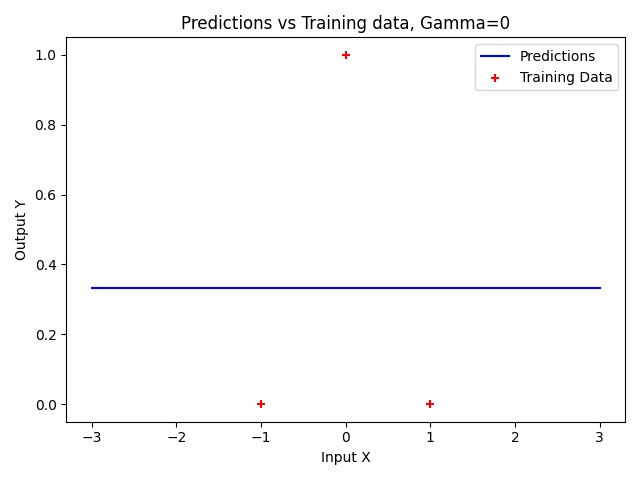
\includegraphics[width=8cm]{kn1.png}}}
\qquad
\subfloat[Gamma = 1]{{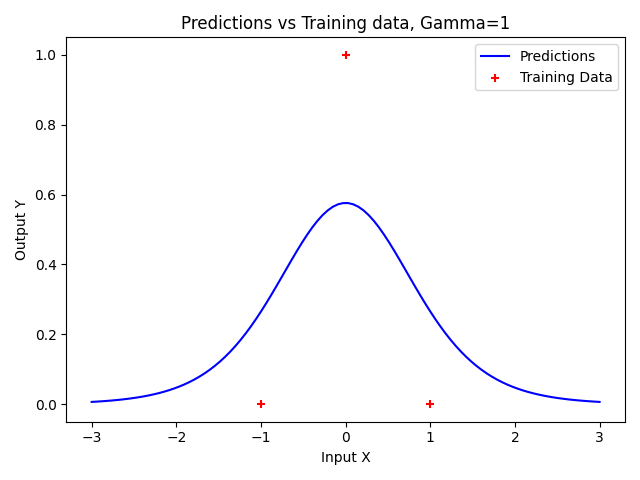
\includegraphics[width=8cm]{kn2.png}}}
\qquad
\subfloat[Gamma = 5]{{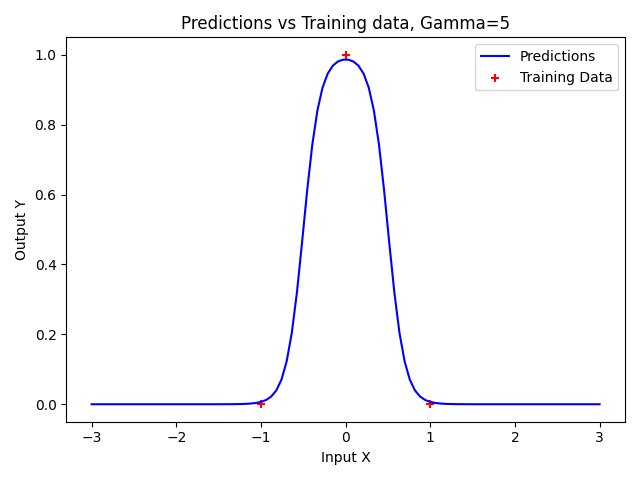
\includegraphics[width=8cm]{kn3.png}}}
\qquad
\subfloat[Gamma = 10]{{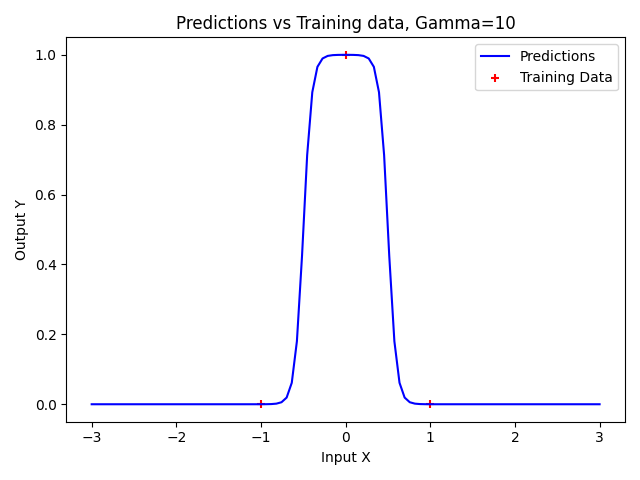
\includegraphics[width=8cm]{kn4.png}}}
\qquad
\subfloat[Gamma = 25]{{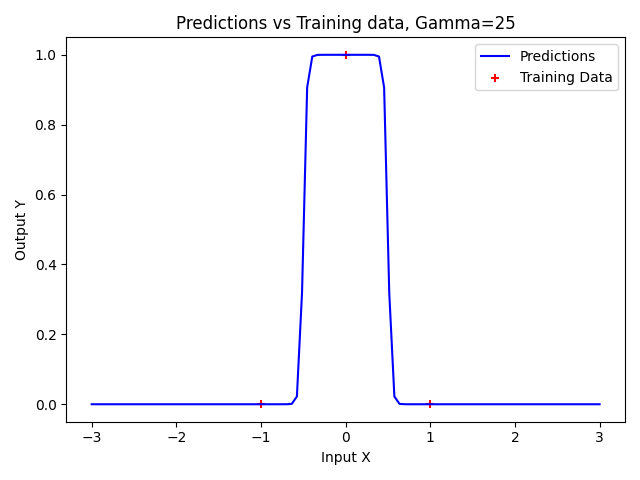
\includegraphics[width=8cm]{kn5.png}}}
\end{figure}
From the above figures we can see that as we increase gamma, our predictions fit closer to the training data,  with low values of data underfitting the data such as when gamma = 1 and higher values of gamma confirming very closely to the data such as when gamma = 25.

\subsection{B}
From the graphs in A we can see our predictions changing as we increase the value of Gamma. This is due to fact that as we increase gamma, we decrease the rate at which the out put for our kernel grows. KNN uses the distances between a point and all other points in the data and selects the K closest examples, then sets the averages of the labels. Normally all datapoints have uniform weights but by using a gaussian kernel, the weights of datapoints changes as they get further away from the origin datapoint, with gamma effecting how quickly this change happens. From our data we can see that small values of Gamma make the kernel decrease much slower with distance and underfit the data, hence the slopes we see when Gamma = 1, due to less weight being on points from the origin point. In contrast, high values of Gamma make the kernel decrease very quickly, putting more weight on points even if they're very close to the origin, causing the preditions to snap towards the nearest datapoint such as when Gamma = 25. This also explains why when x is between -.5 and .5 we see y =1 as it's snapping towards the nearest data point. 

\subsection{C}
From the graphs below, we can see that as we change C and the Gamma, the shape of our graph alters quite considerably. Higher C values gives graphs with higher peaks and with higher gamma values influencing this also. 
\\ The below values represent each page of graphs hence the blocks of 5.

\begin{figure}[h]
\centering
\subfloat[Gamma = 0, C = 0.1]{{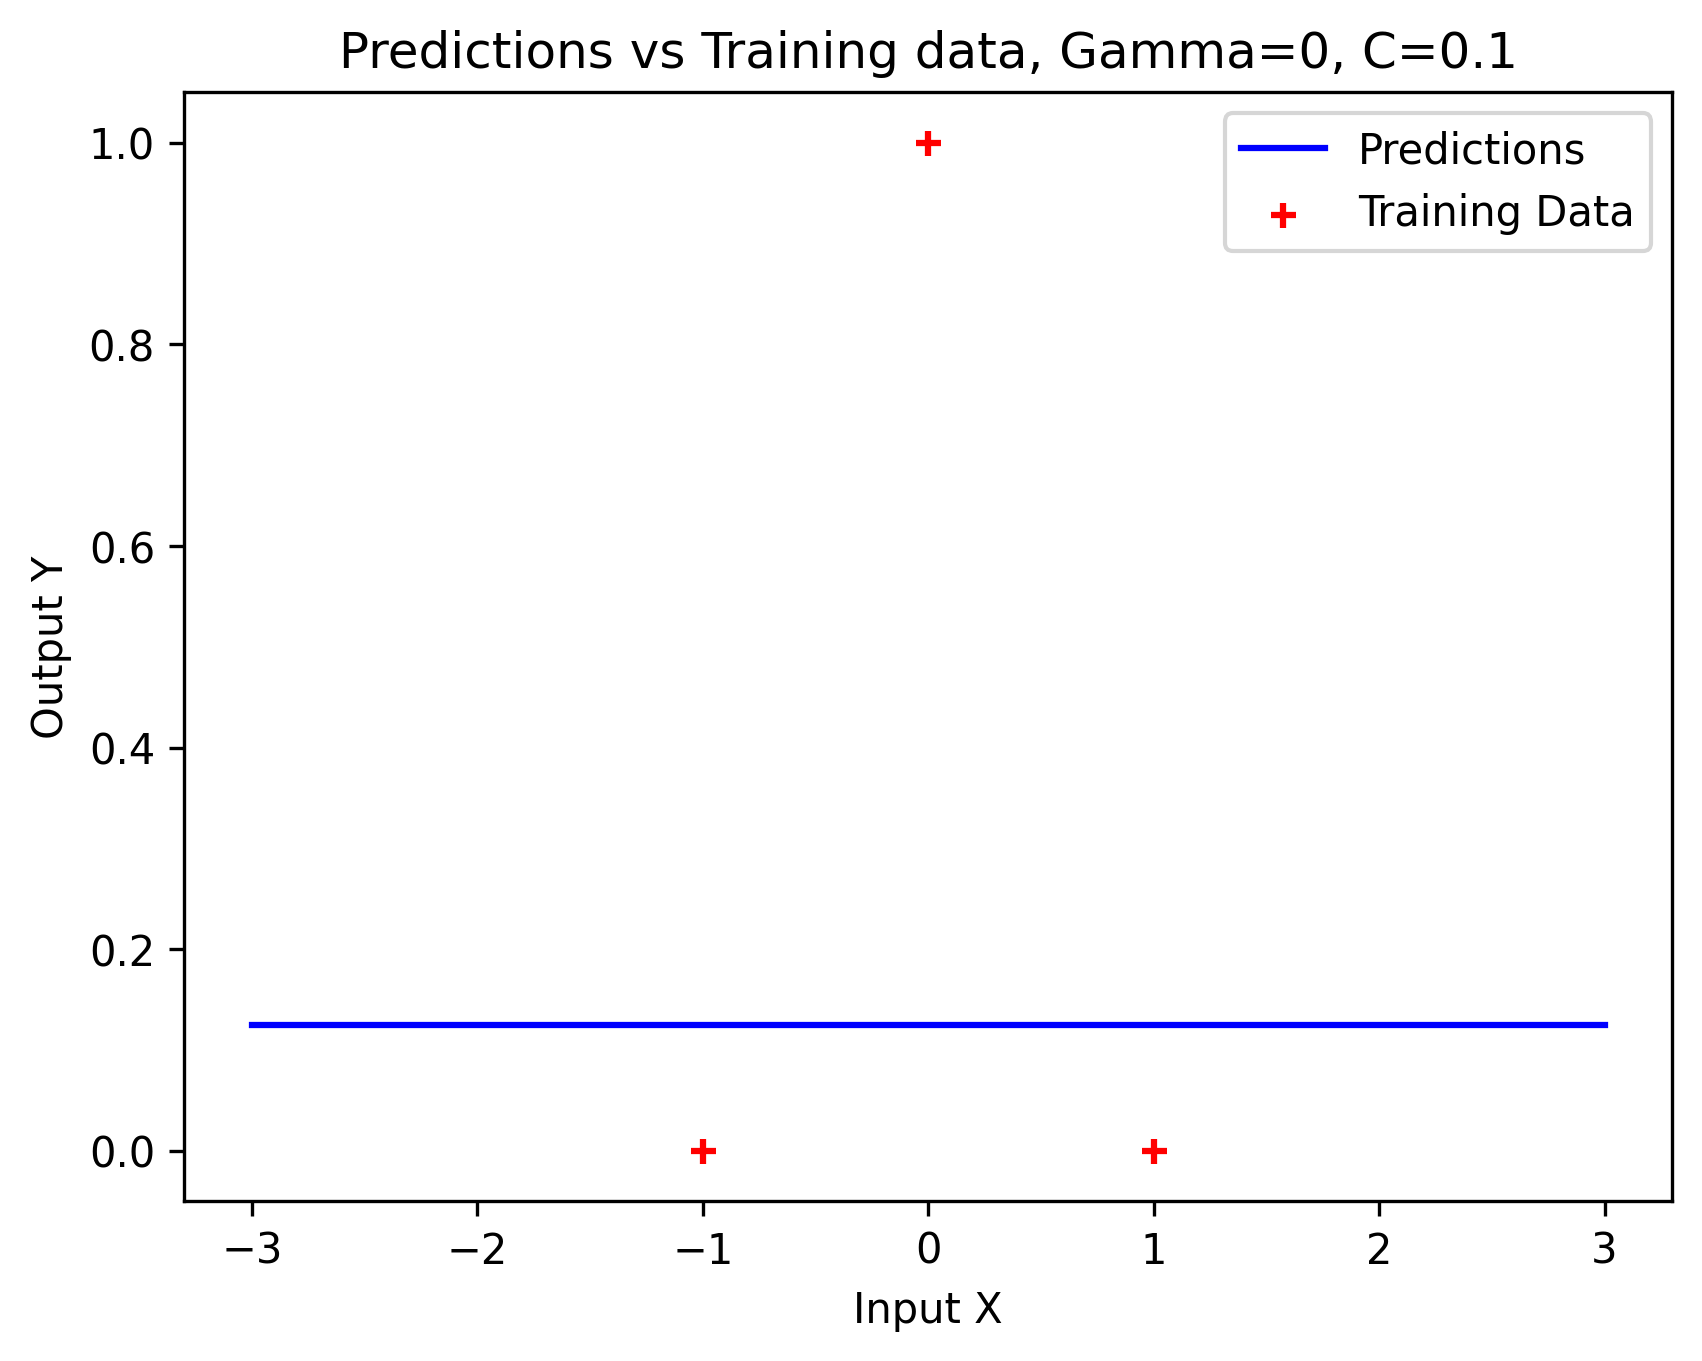
\includegraphics[width=8cm]{kr00.png}}}
\qquad
\subfloat[Gamma = 1, C = 0.1]{{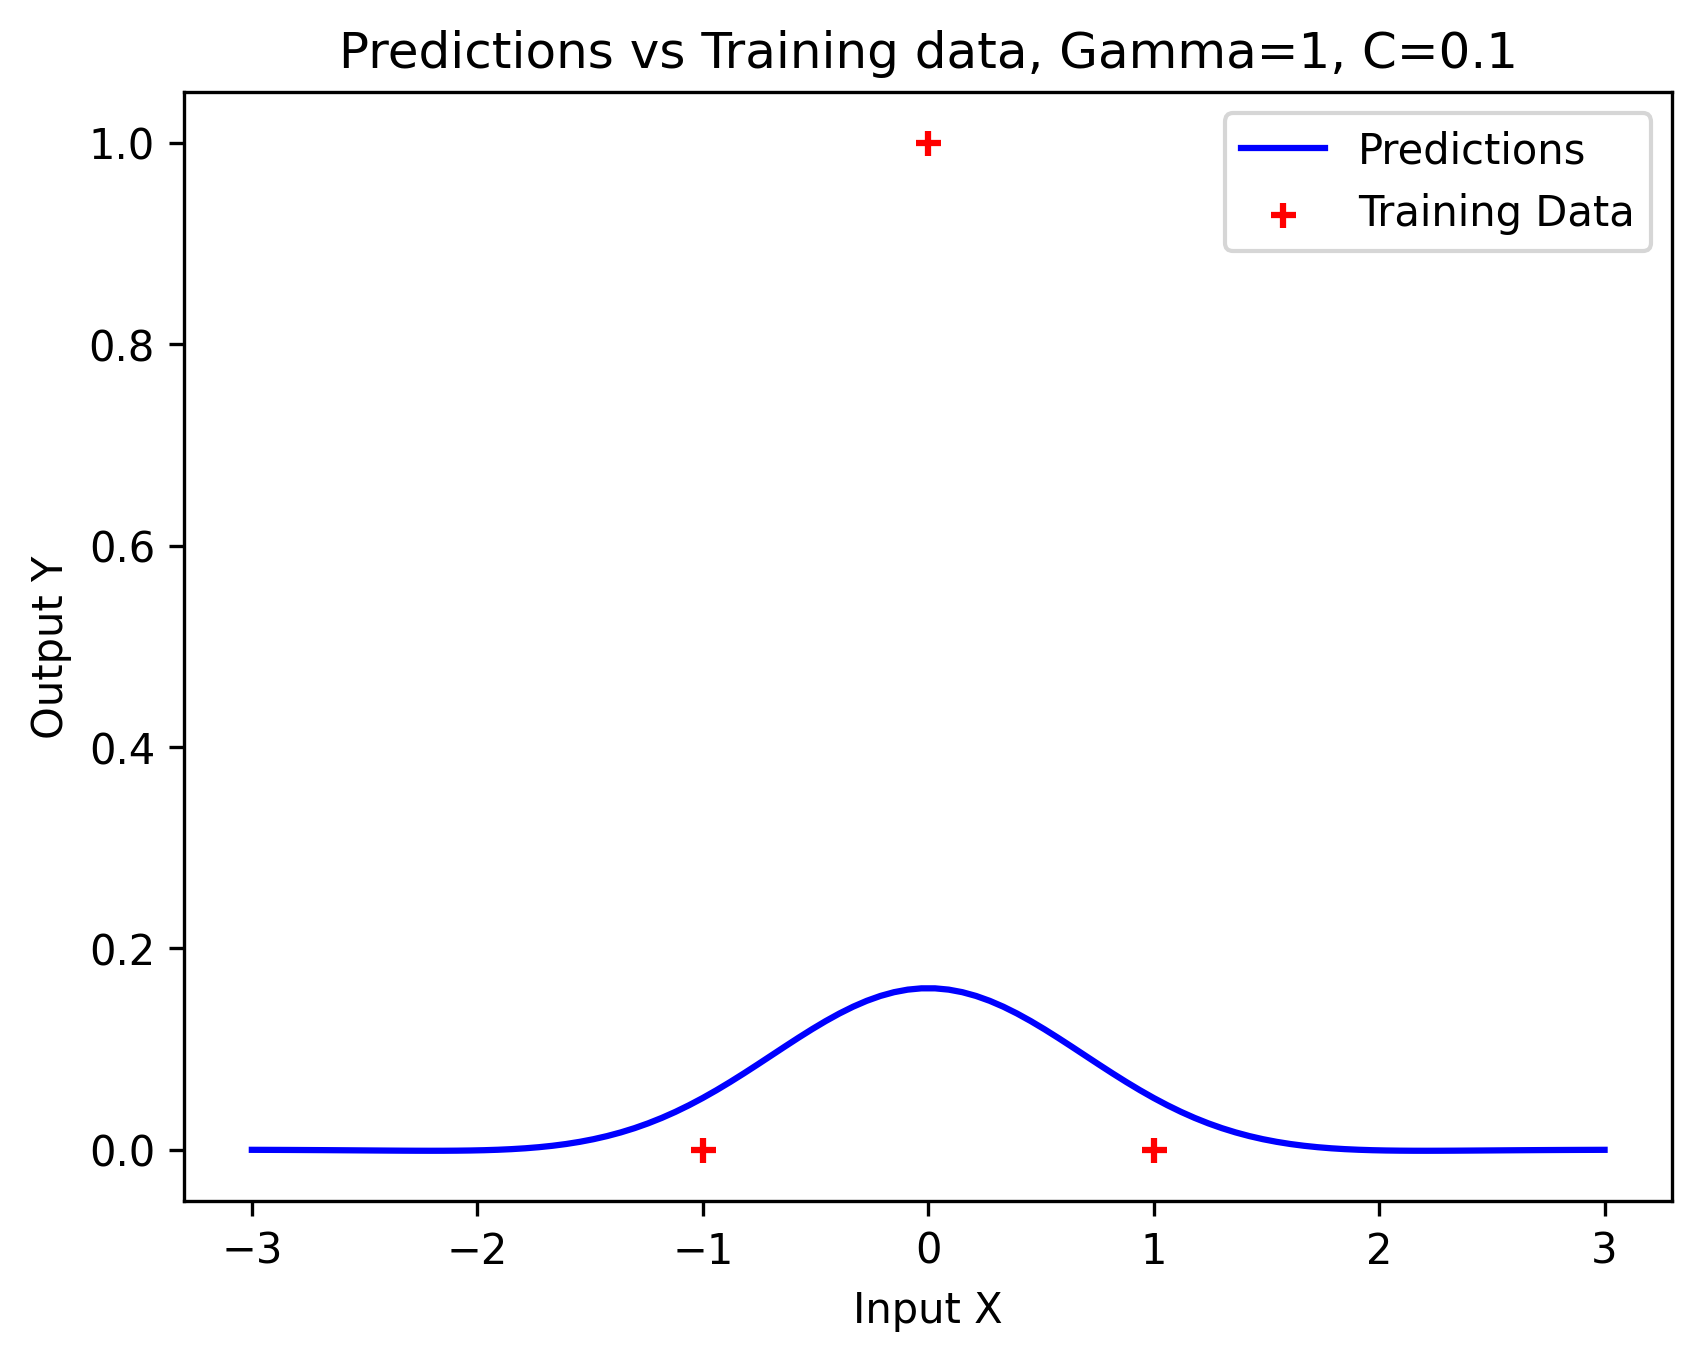
\includegraphics[width=8cm]{kr01.png}}}
\qquad
\subfloat[Gamma = 5, C= 0.1]{{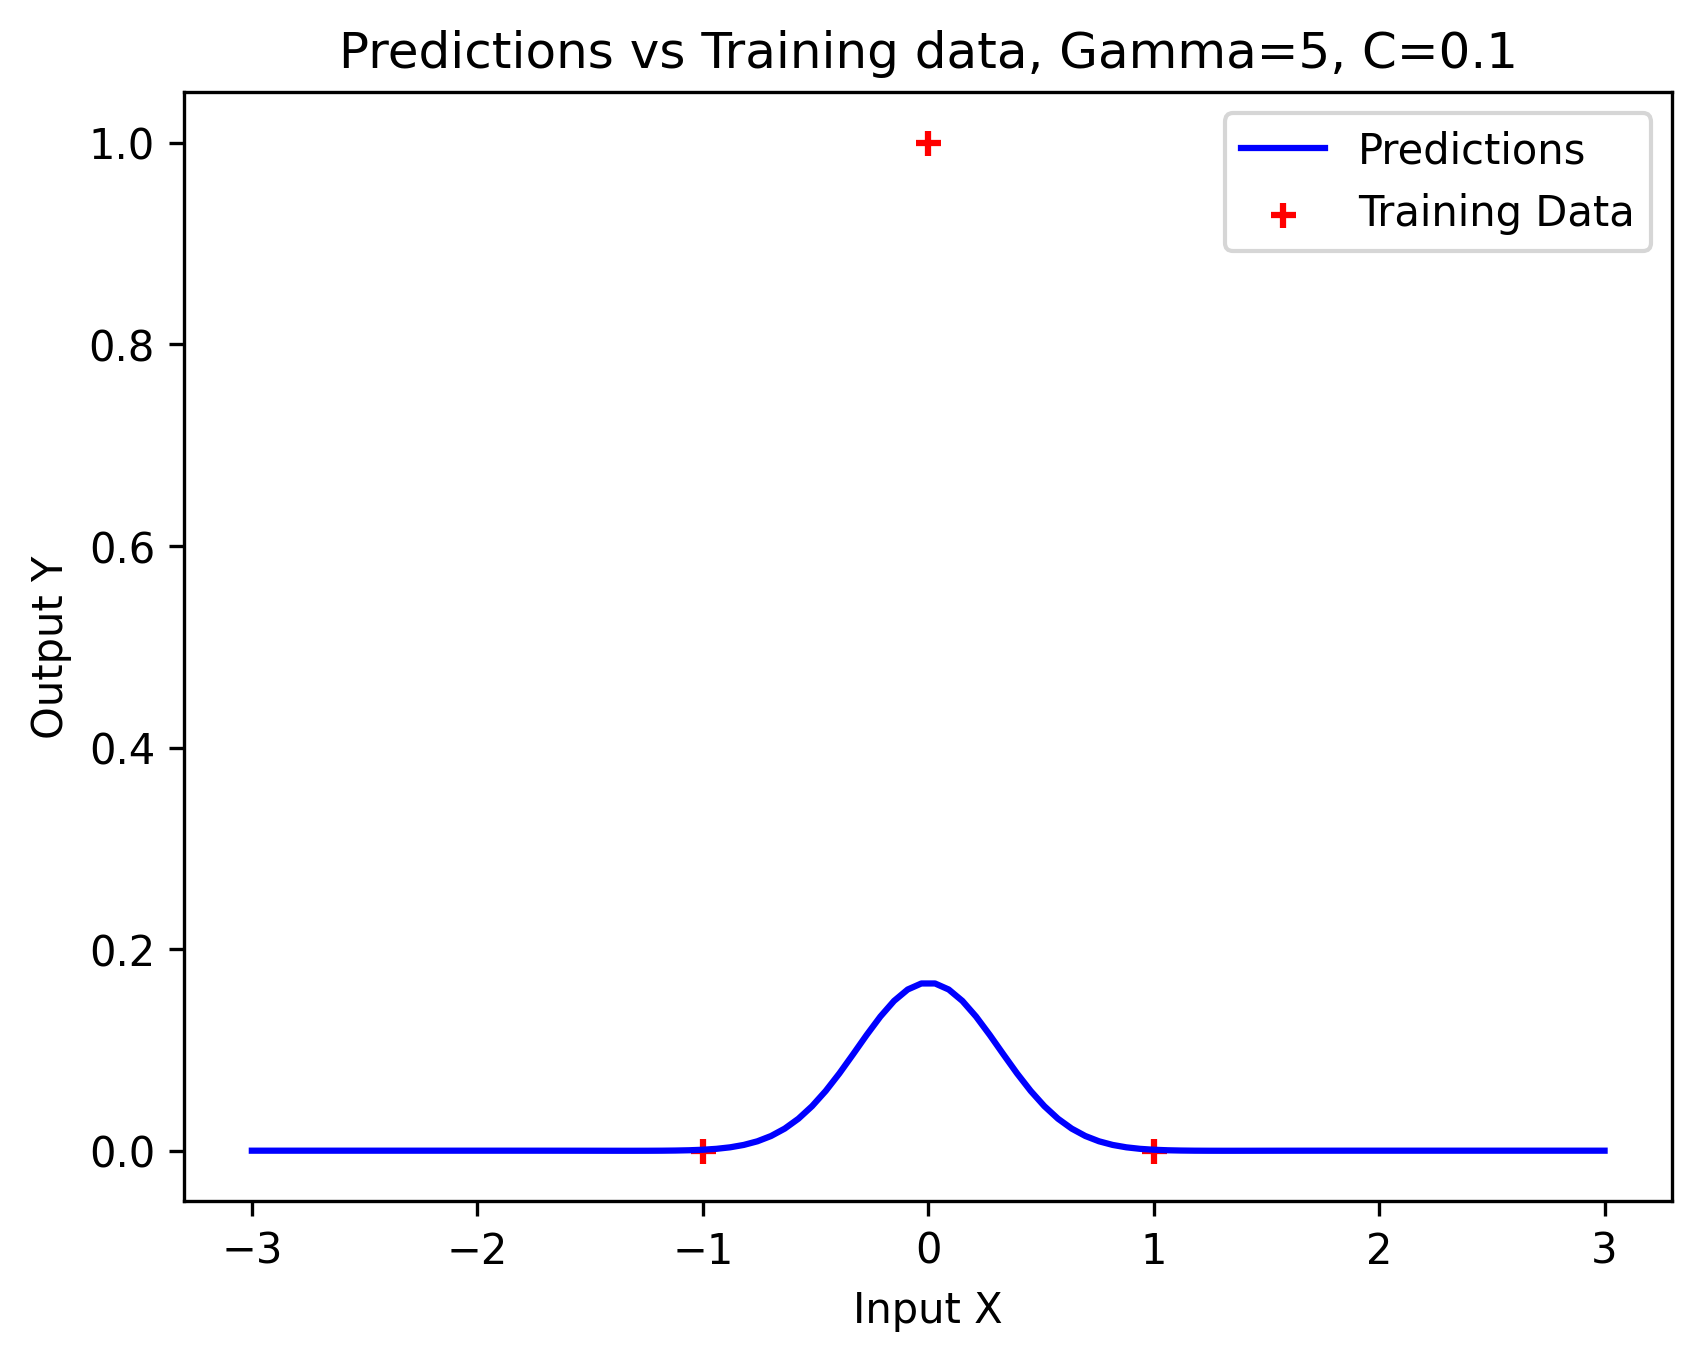
\includegraphics[width=8cm]{kr02.png}}}
\qquad
\subfloat[Gamma = 10, C= 0.1]{{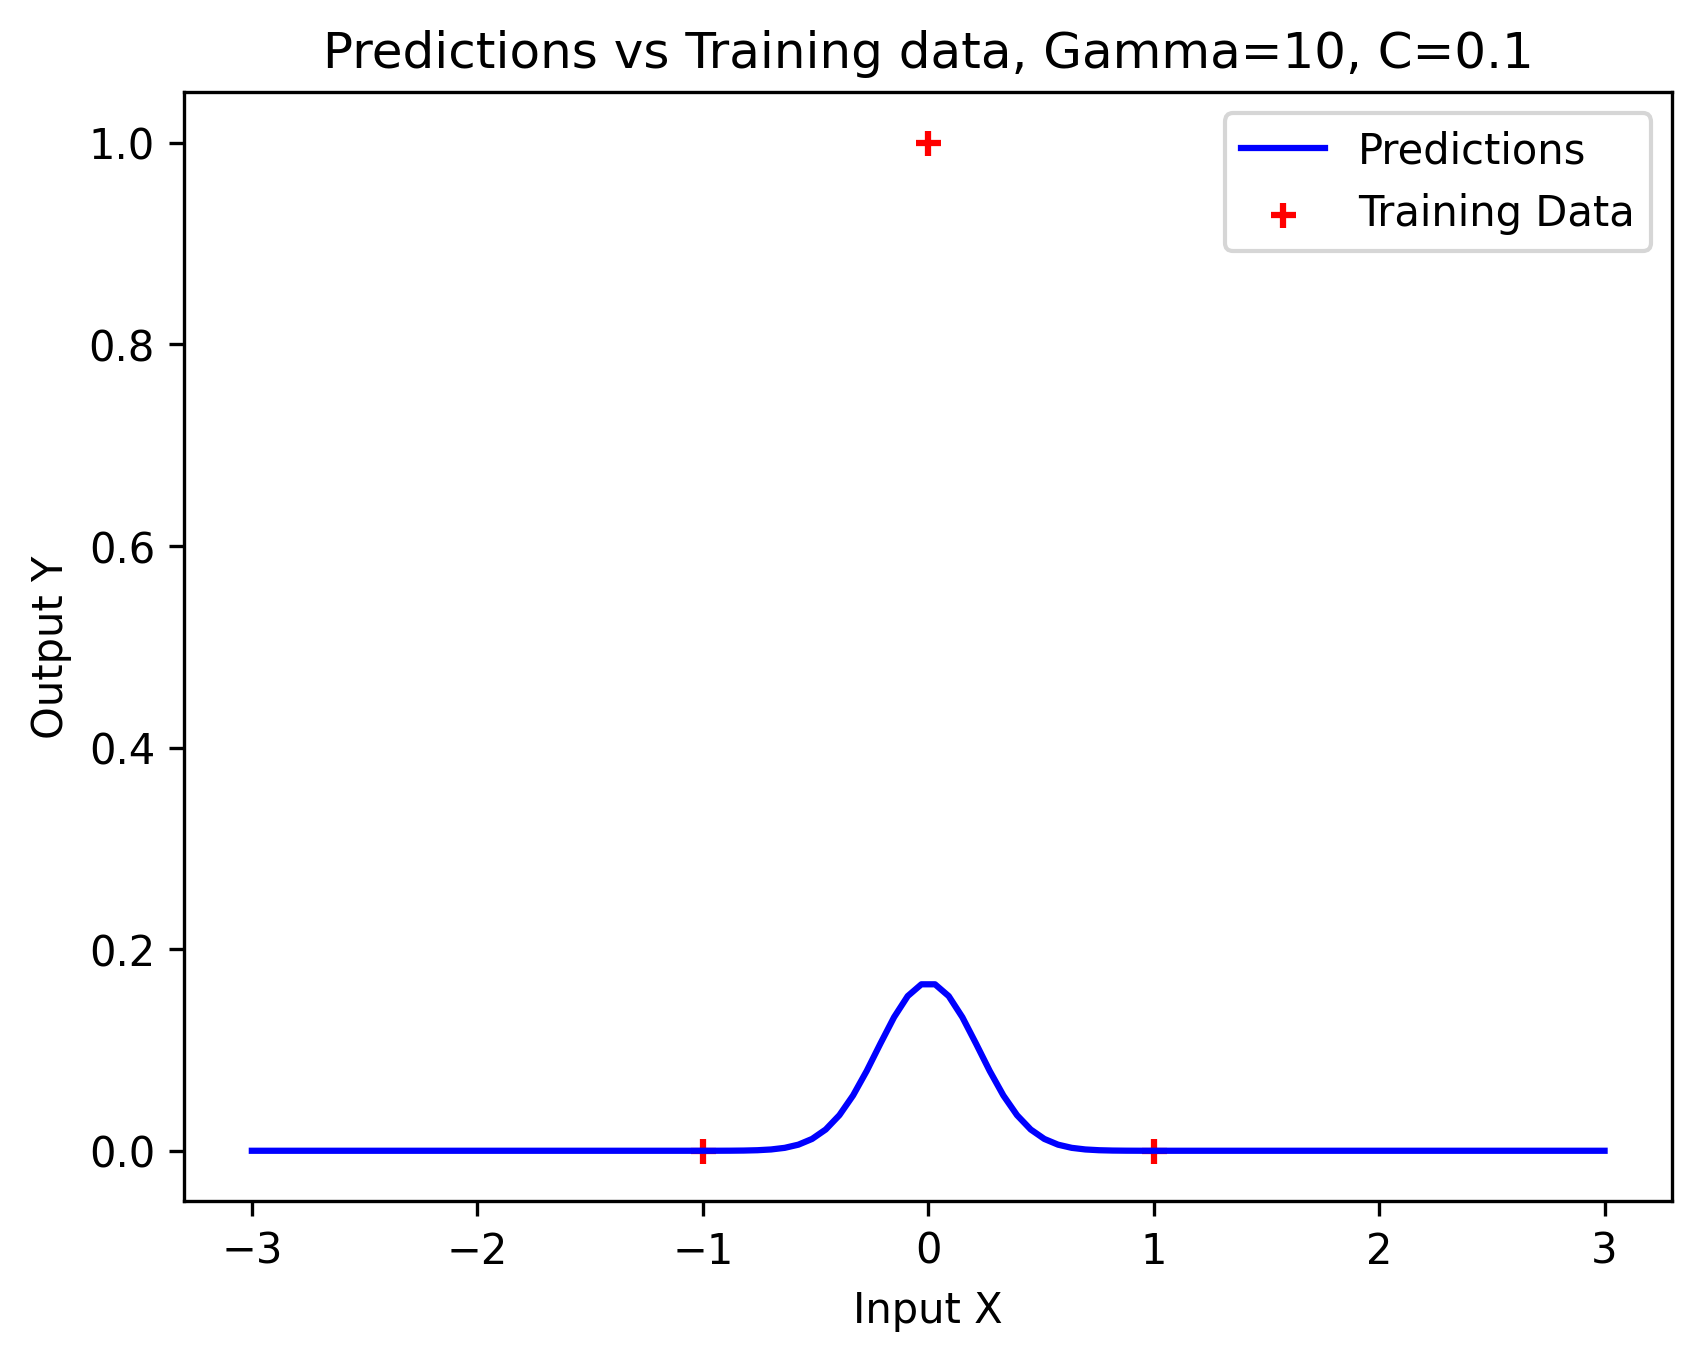
\includegraphics[width=8cm]{kr03.png}}}
\qquad
\subfloat[Gamma = 25, C= 0.1]{{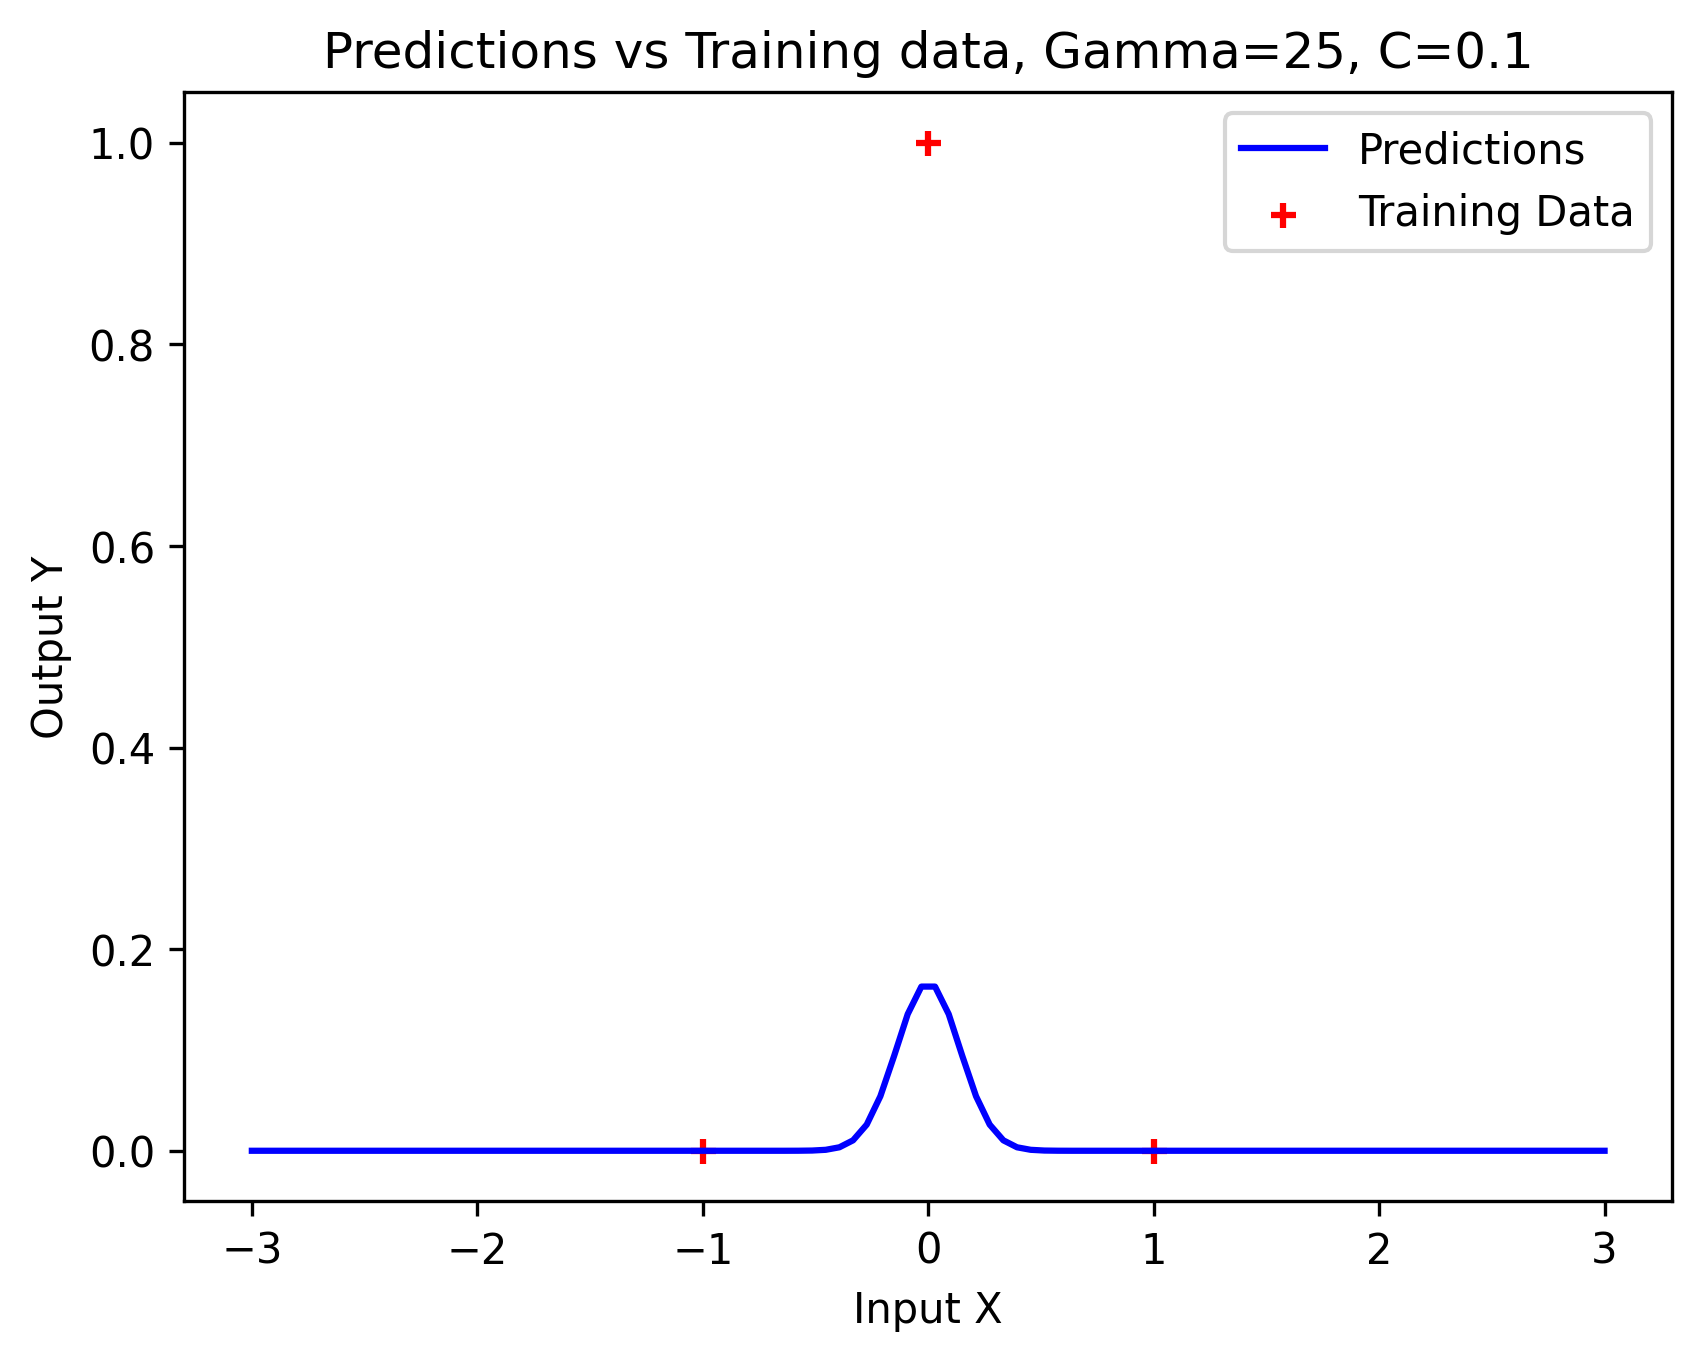
\includegraphics[width=8cm]{kr04.png}}}
\end{figure}
\(\theta_0 = -0.025, \theta_1= 0.175 , \theta_2= -0.025\)\\
\(\theta_0= -0.0103, \theta_1= 0.1679 , \theta_2 =-0.0103\)\\
\(\theta_0 =-0.0002, \theta_1= 0.1667 , \theta_2 =-0.0002\)\\
\(\theta_0 =-0.0, \theta_1 =0.1667 , \theta_2 =-0.0\)\\
\(\theta_0 =-0.0, \theta_1= 0.1667 , \theta_2 =-0.0\)\\

\begin{figure}[h]
\centering
\subfloat[Gamma = 0, C = 1]{{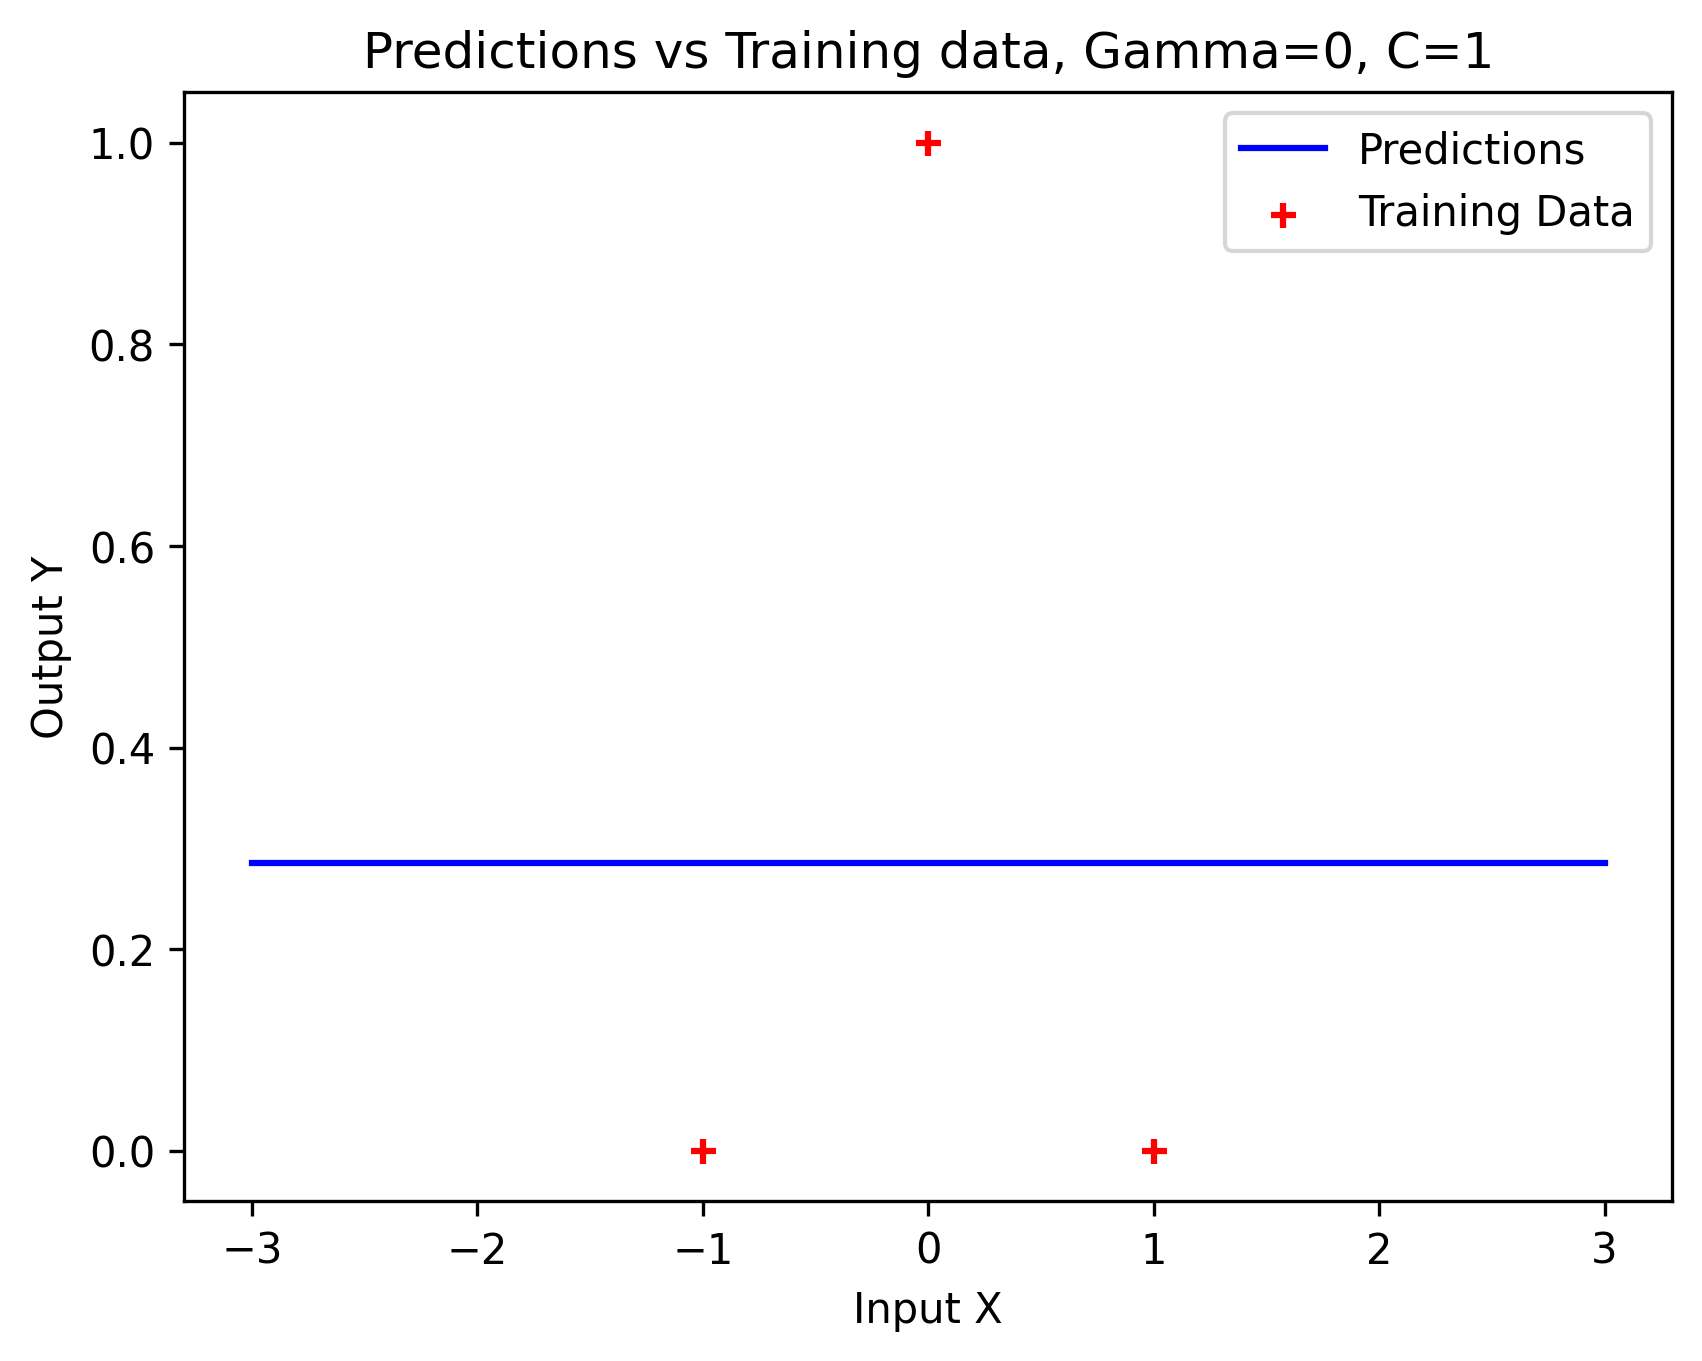
\includegraphics[width=8cm]{kr10.png}}}
\qquad
\subfloat[Gamma = 1, C = 1]{{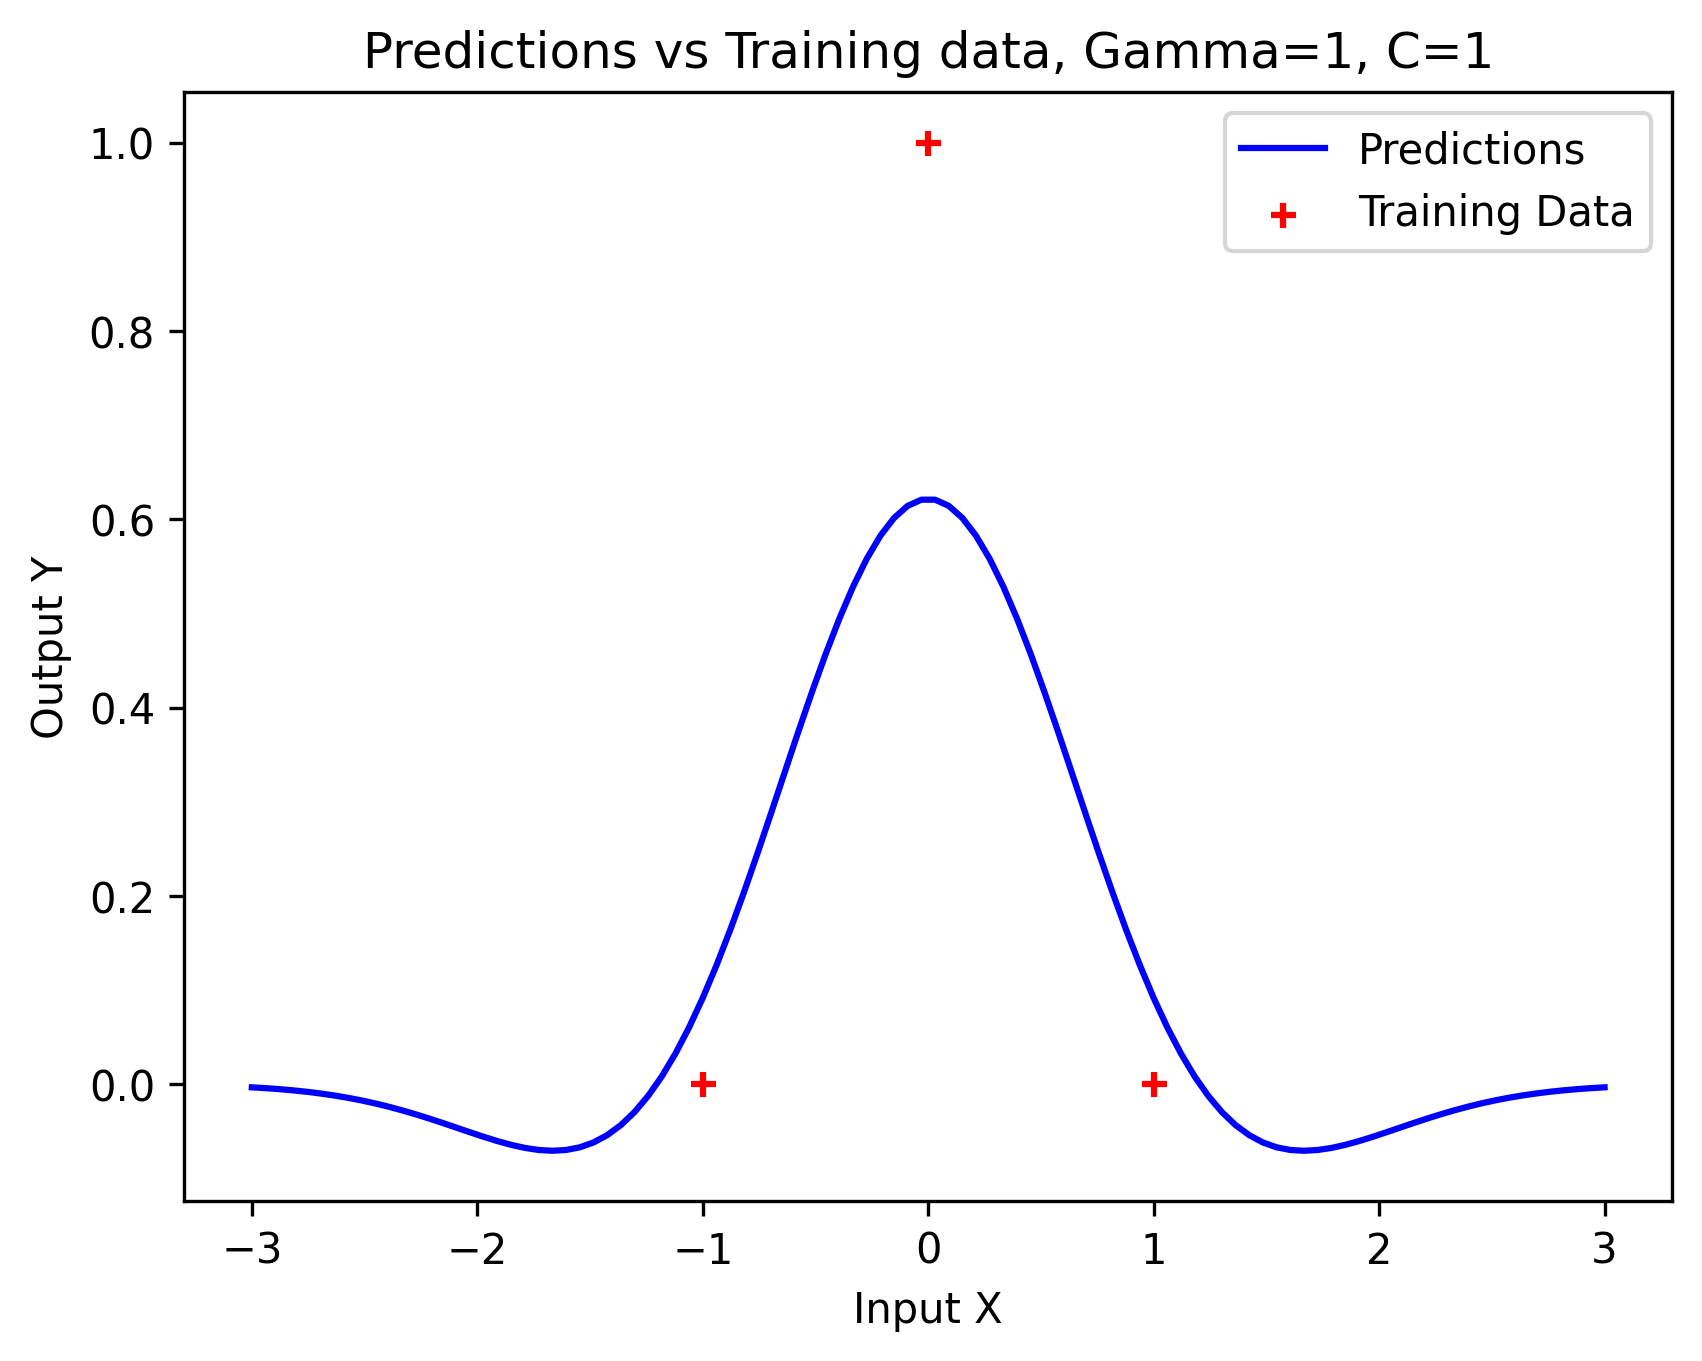
\includegraphics[width=8cm]{kr11.png}}}
\qquad
\subfloat[Gamma = 5, C= 1]{{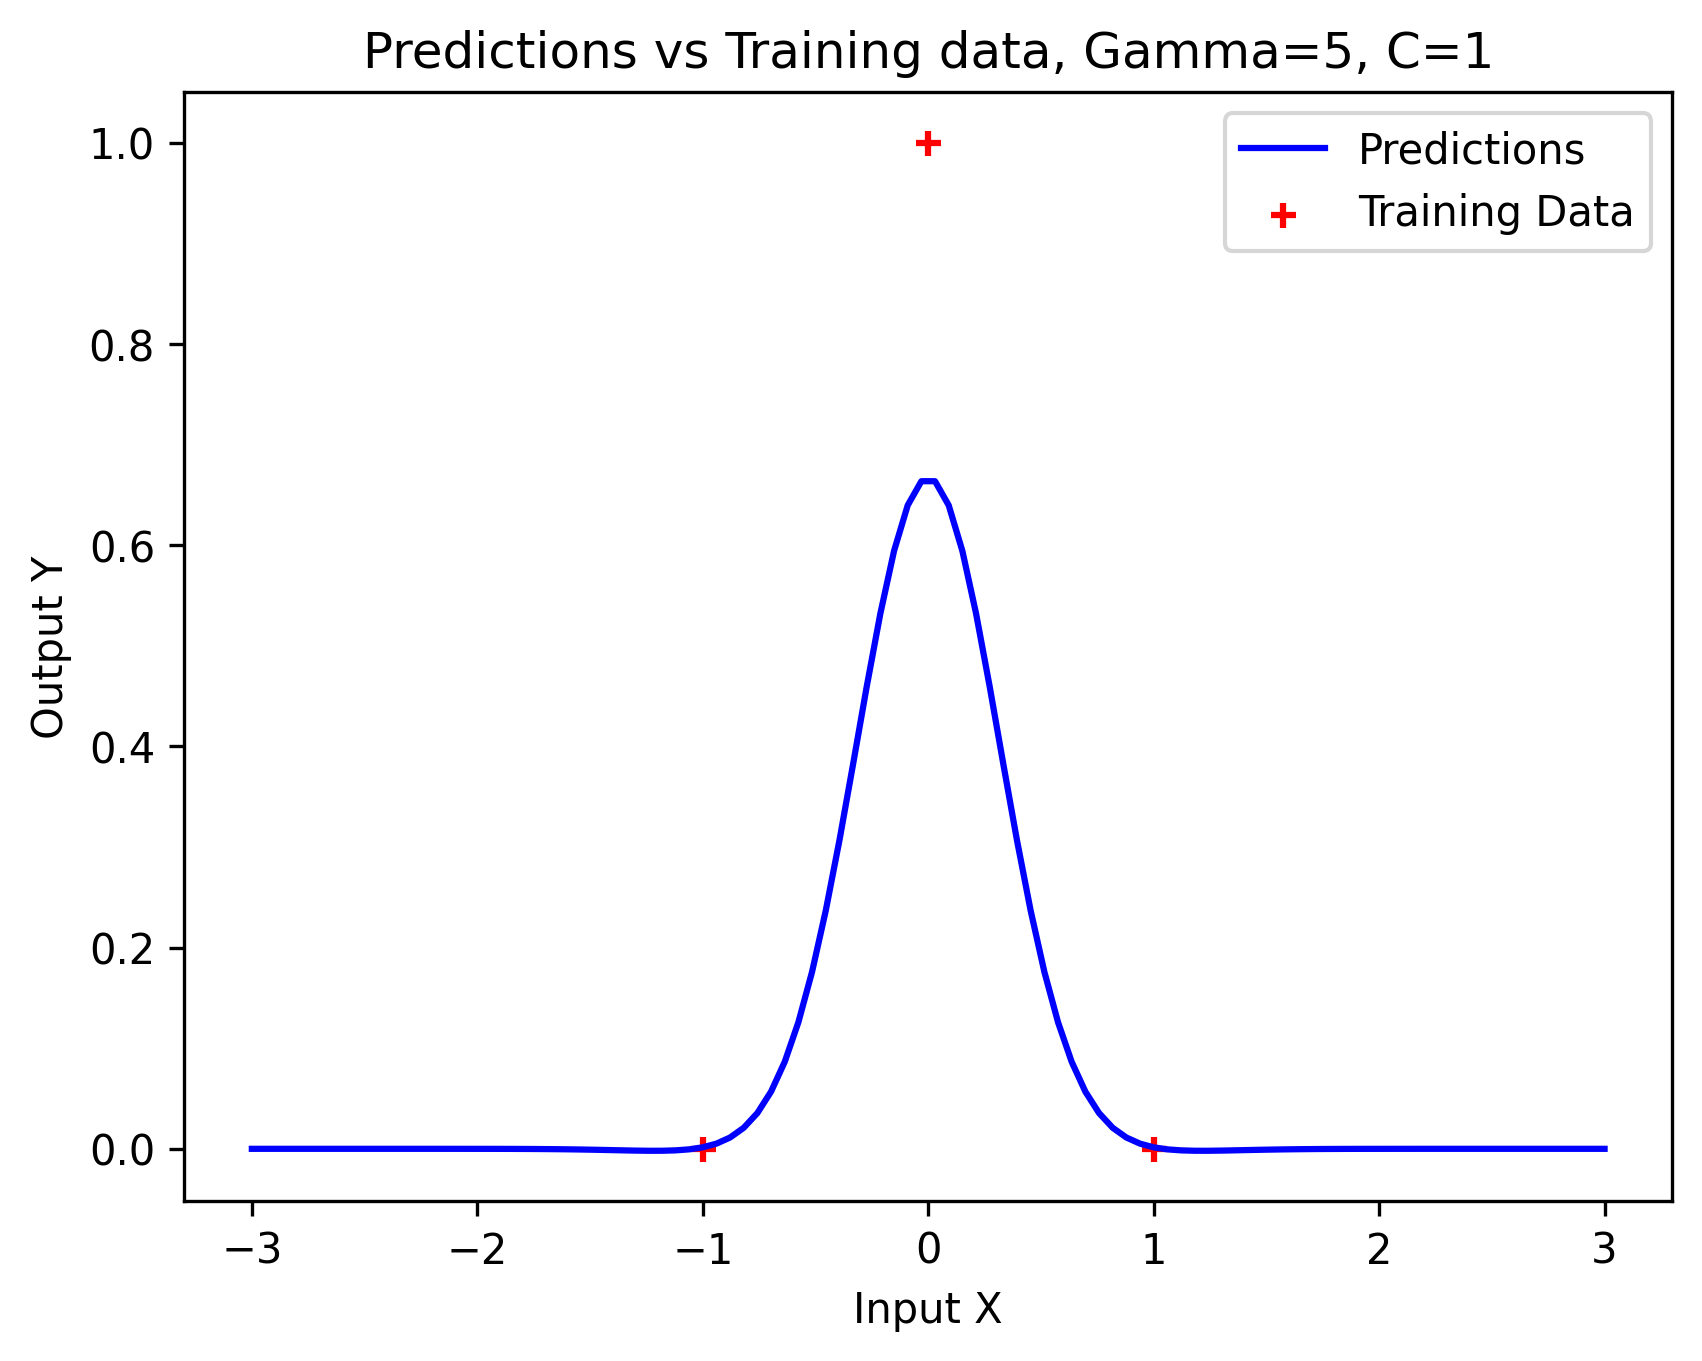
\includegraphics[width=8cm]{kr12.png}}}
\qquad
\subfloat[Gamma = 10, C= 1]{{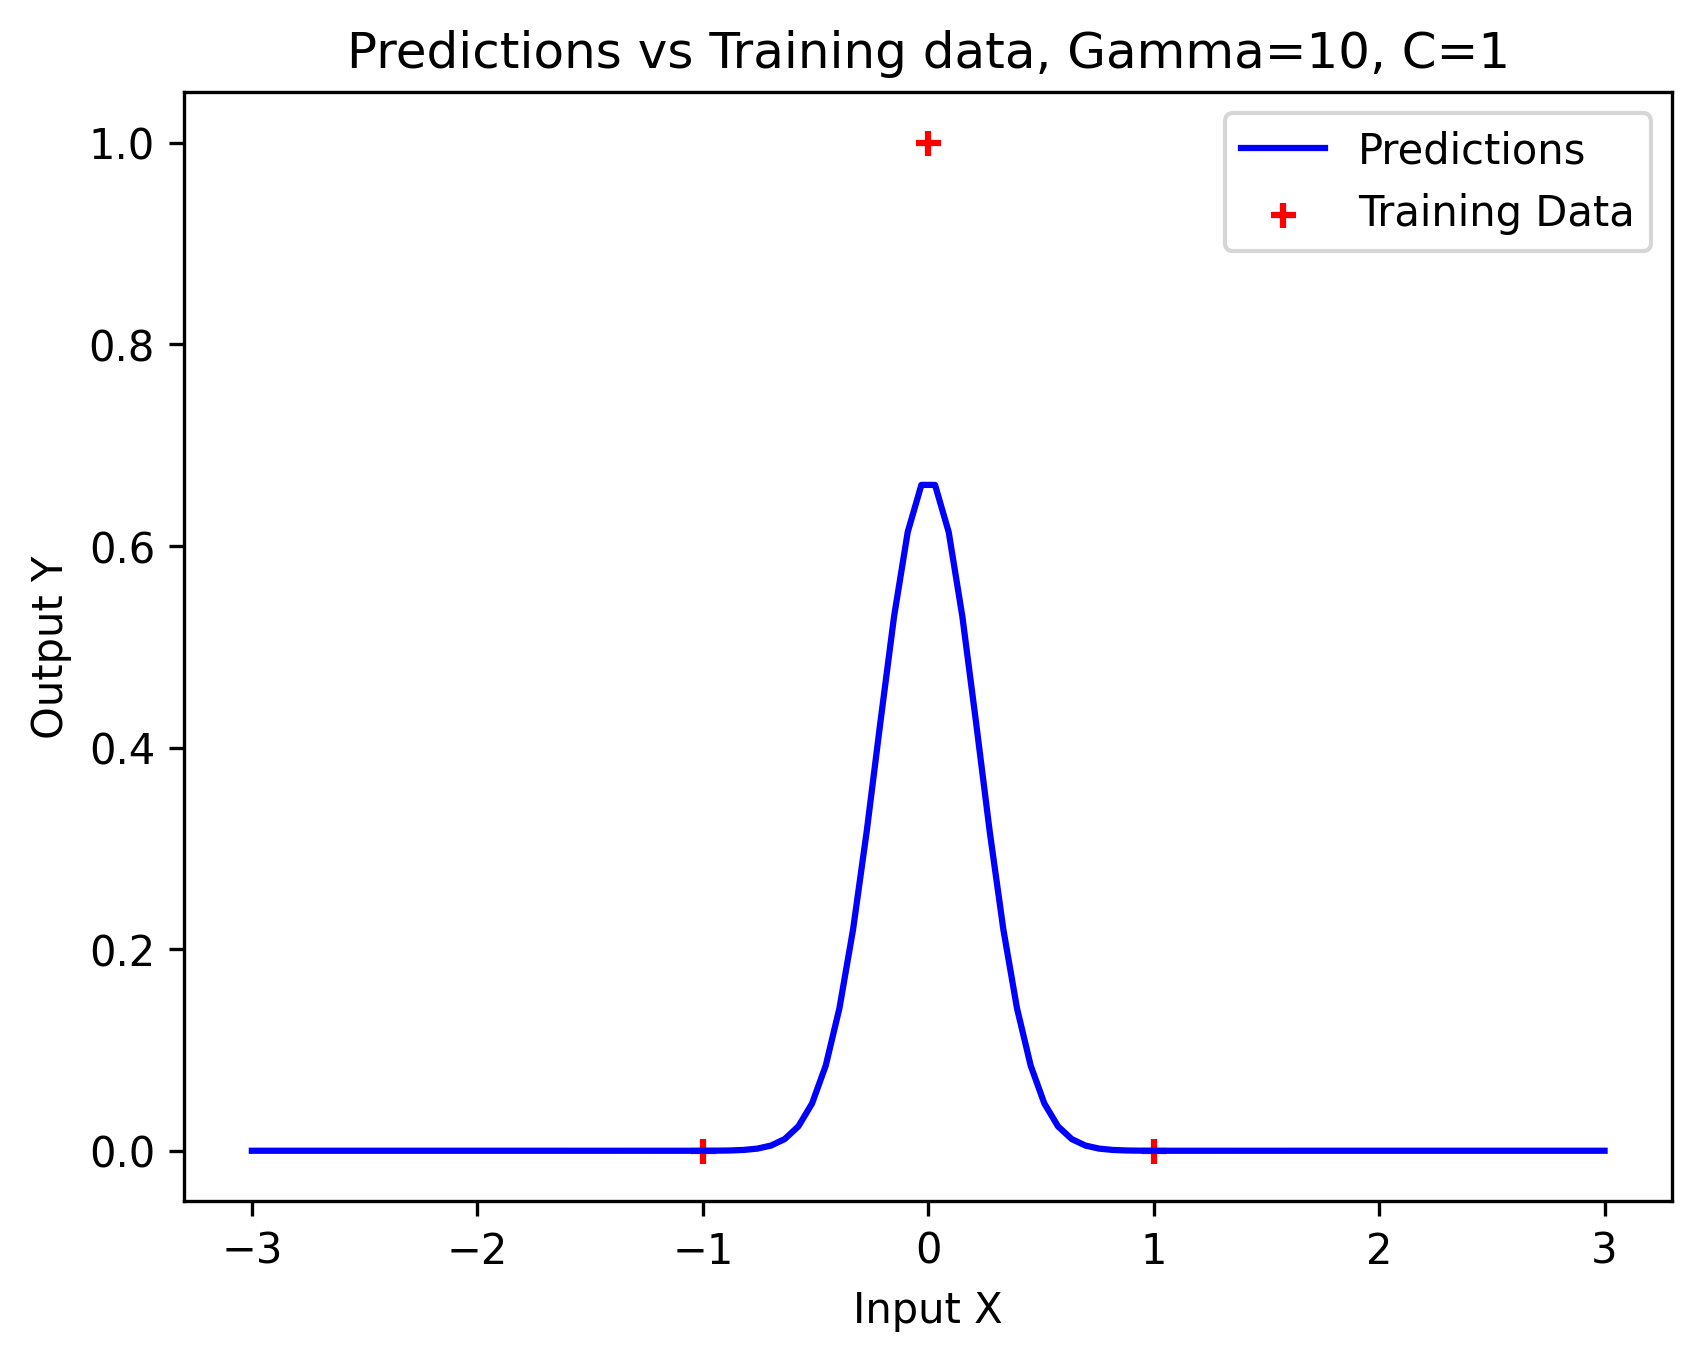
\includegraphics[width=8cm]{kr13.png}}}
\qquad
\subfloat[Gamma = 25, C= 1]{{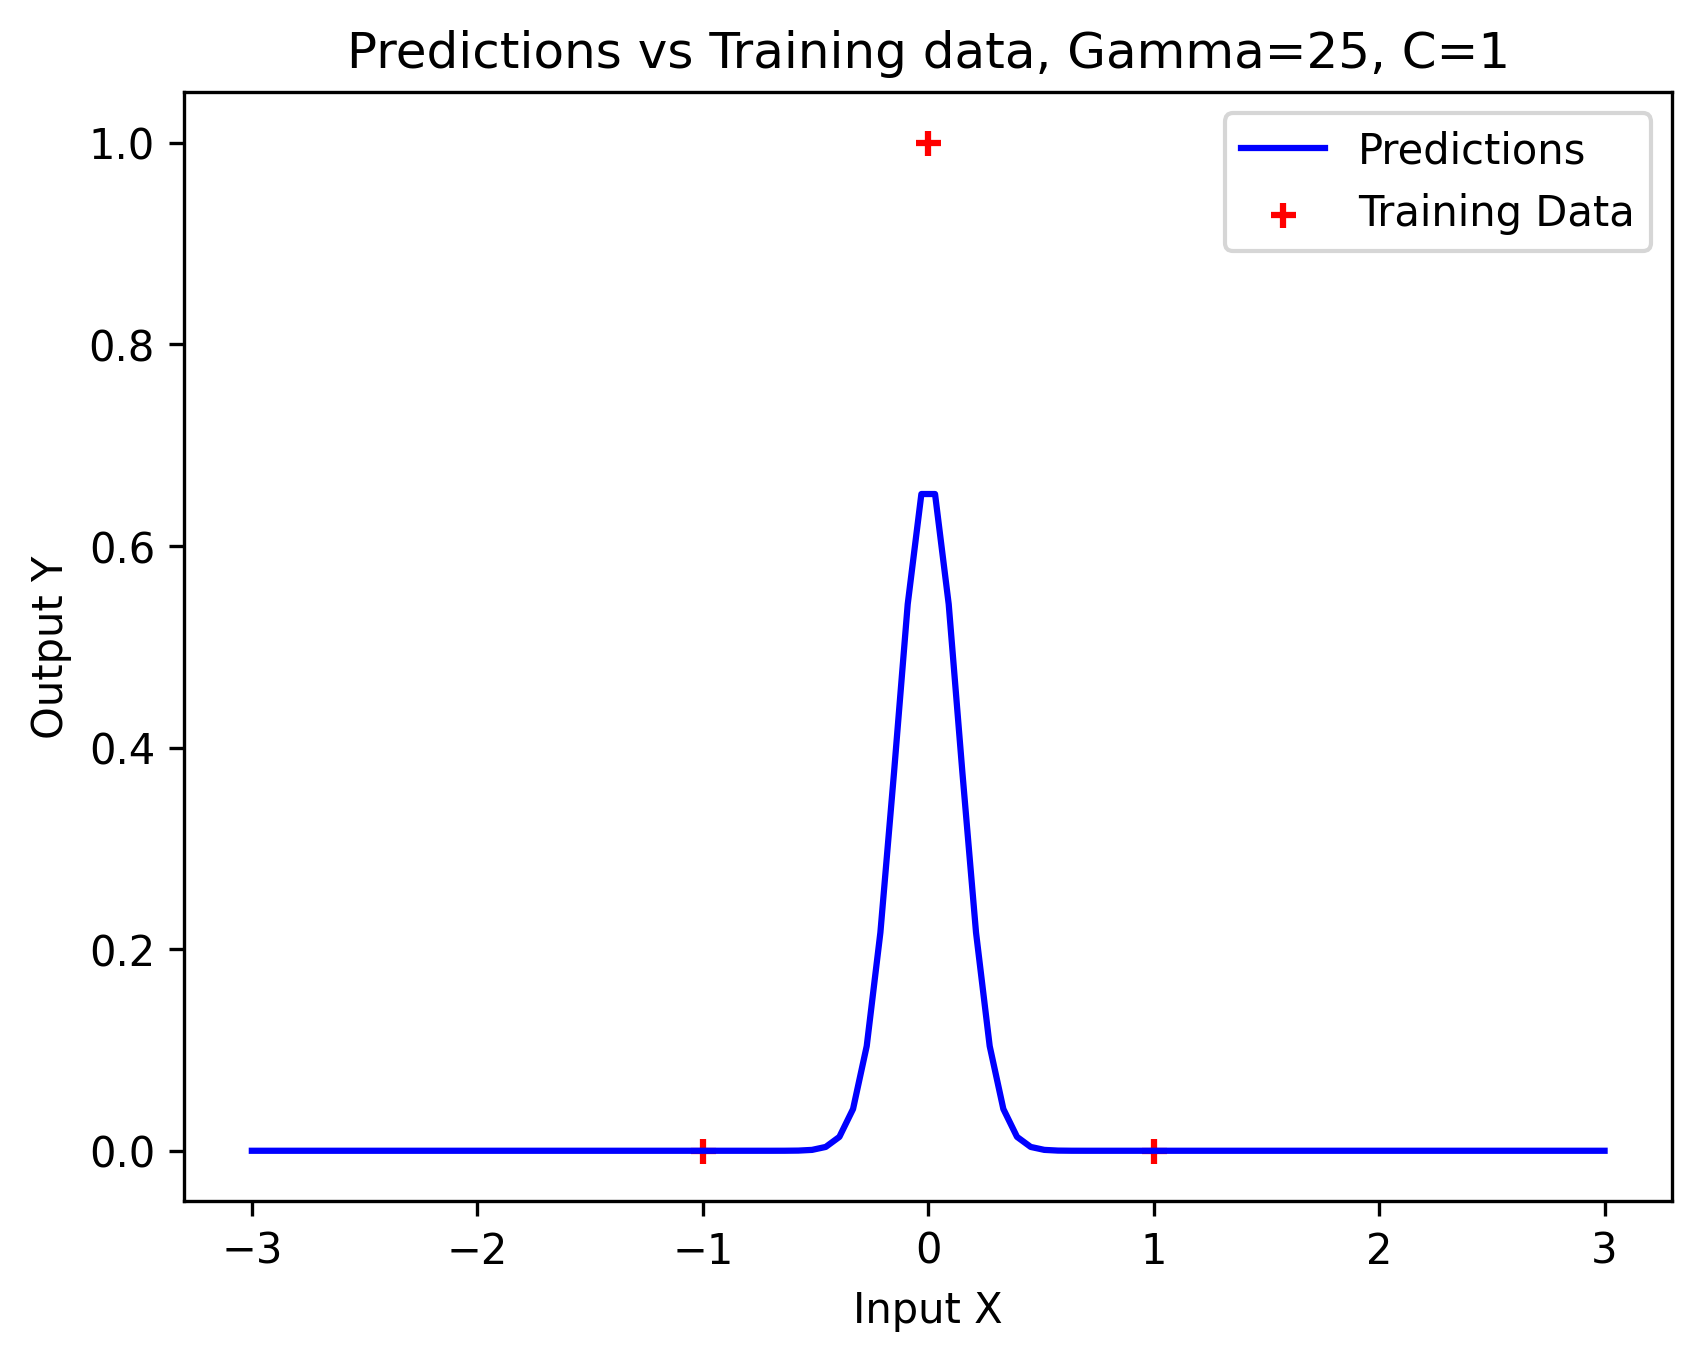
\includegraphics[width=8cm]{kr14.png}}}
\end{figure}
\(\theta_0= -0.5714, \theta_1= 1.4286 , \theta_2 =-0.5714\)\\
\(\theta_0 =-0.1833, \theta_1= 0.7566 , \theta_2 =-0.1833\)\\
\(\theta_0 =-0.003, \theta_1= 0.6667 , \theta_2 =-0.003\)\\
\(\theta_0 =-0.0, \theta_1= 0.6667 , \theta_2= -0.0\)\\
\(\theta_0 =-0.0, \theta_1 =0.6667 , \theta_2 =-0.0\)\\

\begin{figure}[h]
\centering
\subfloat[Gamma = 0, C = 10]{{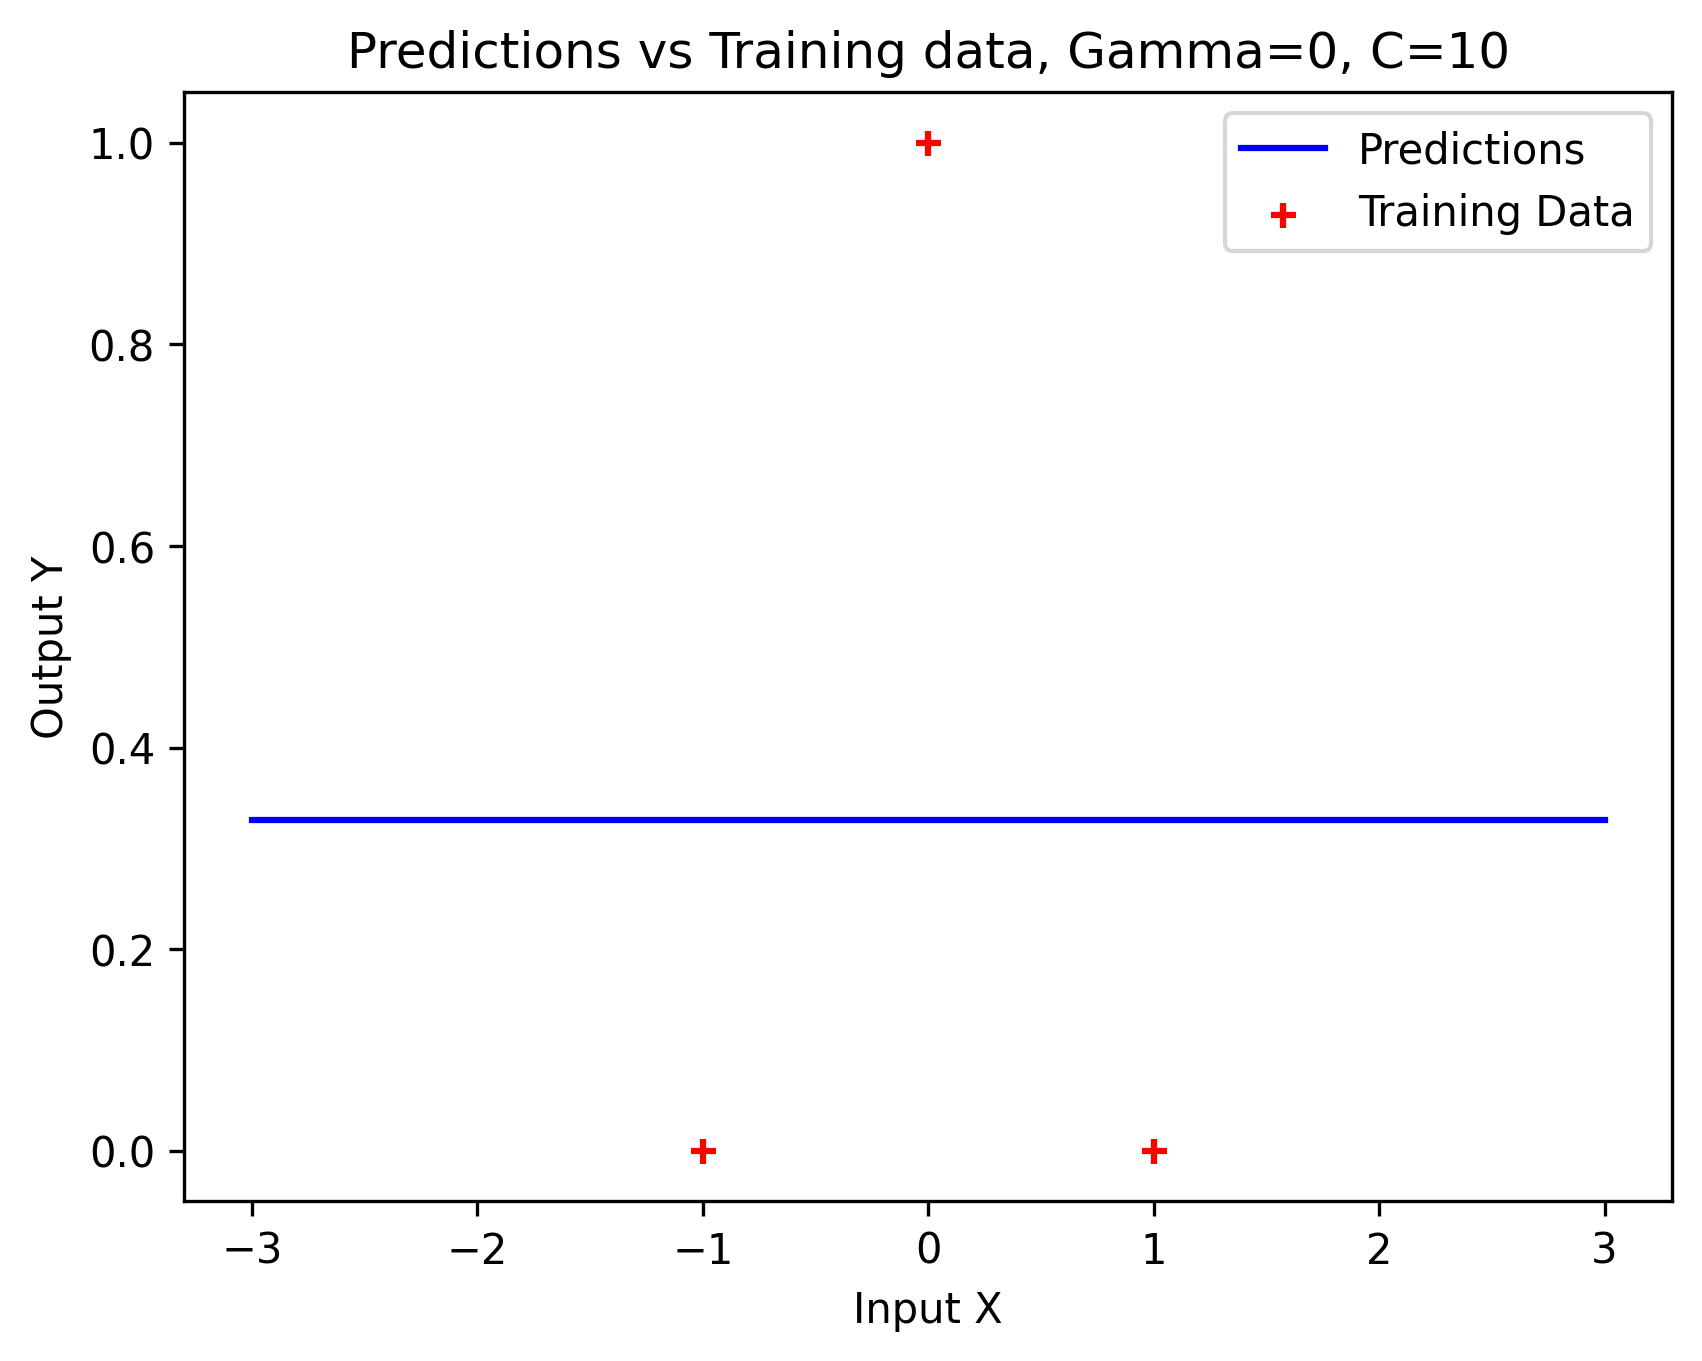
\includegraphics[width=8cm]{kr20.png}}}
\qquad
\subfloat[Gamma = 1, C = 10]{{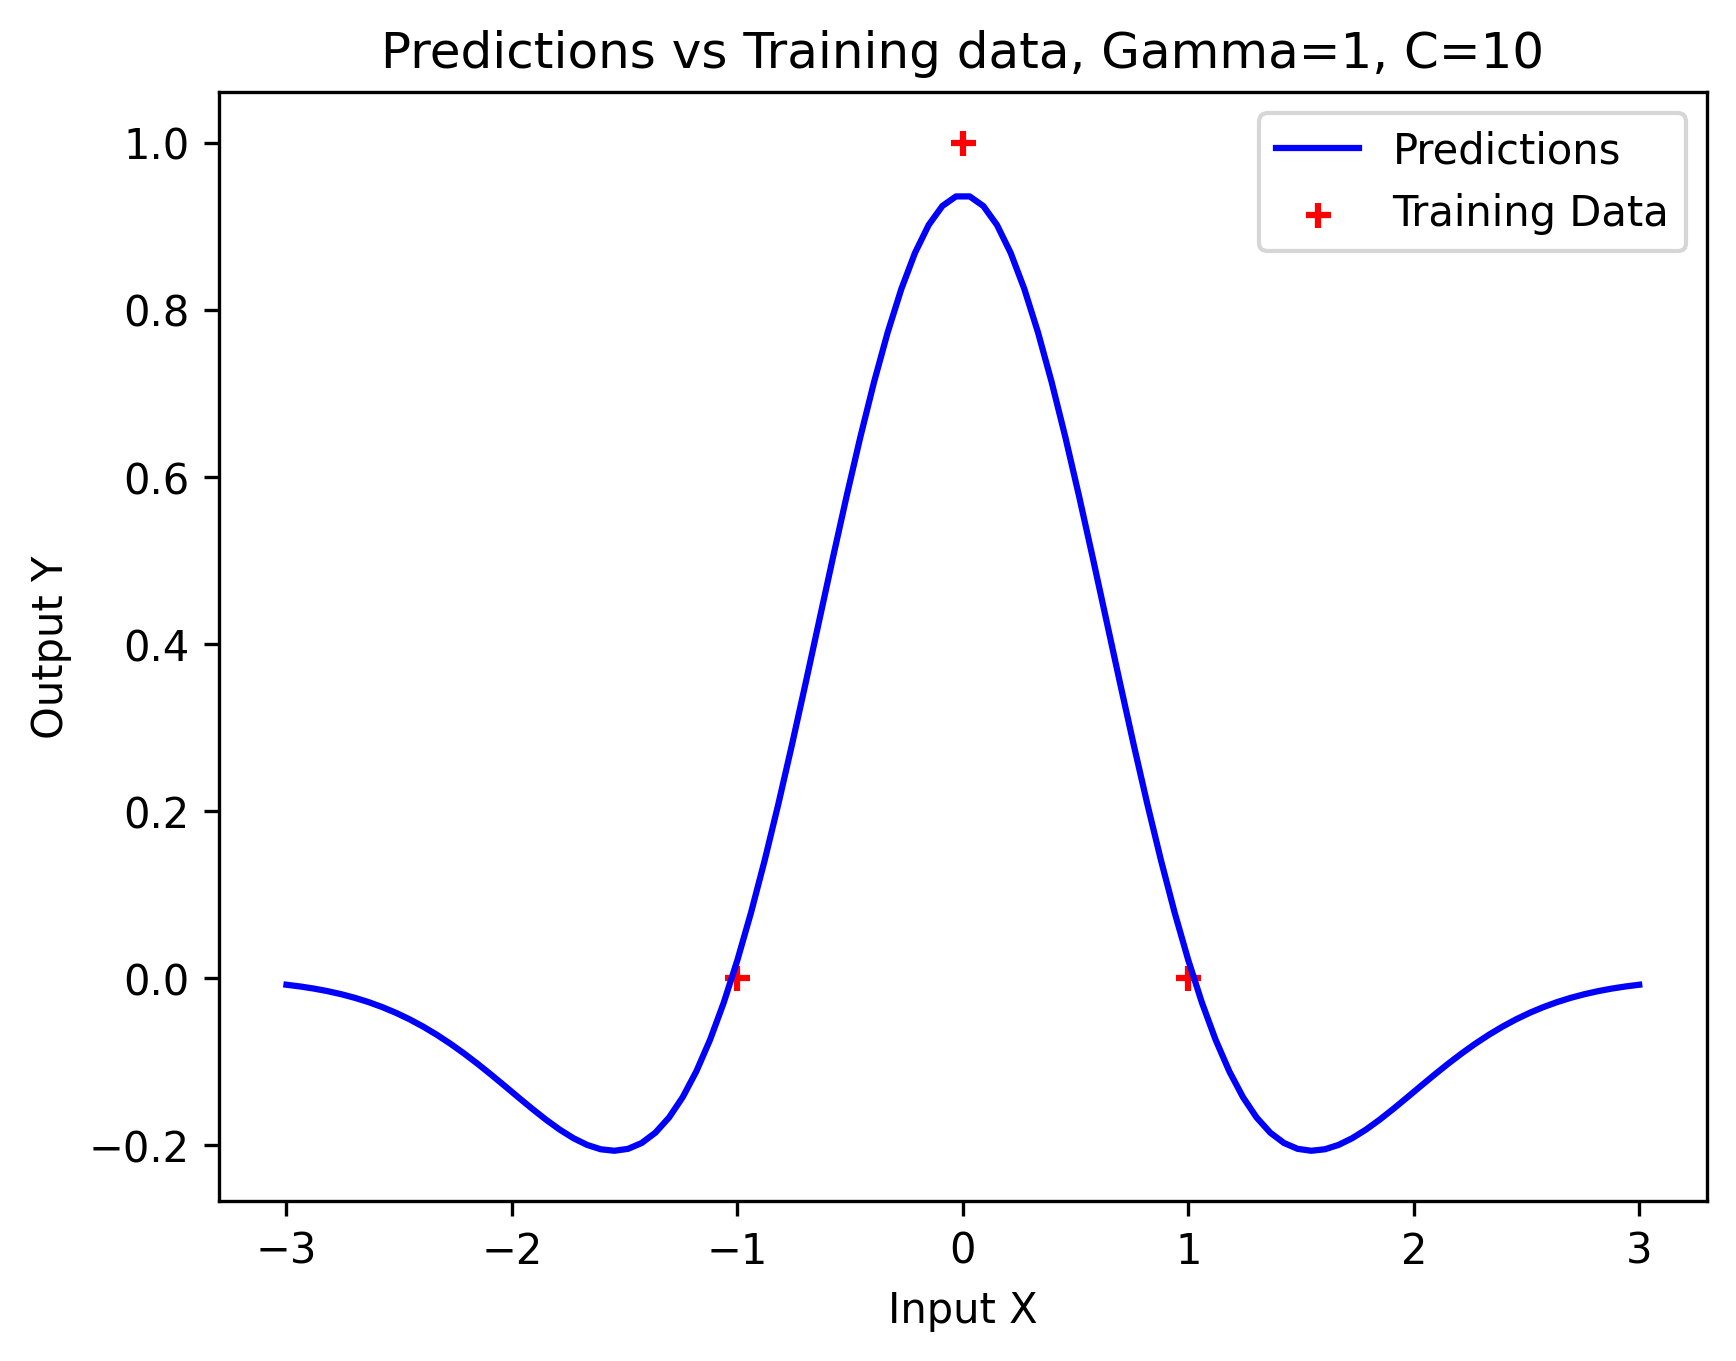
\includegraphics[width=8cm]{kr21.png}}}
\qquad
\subfloat[Gamma = 5, C= 10]{{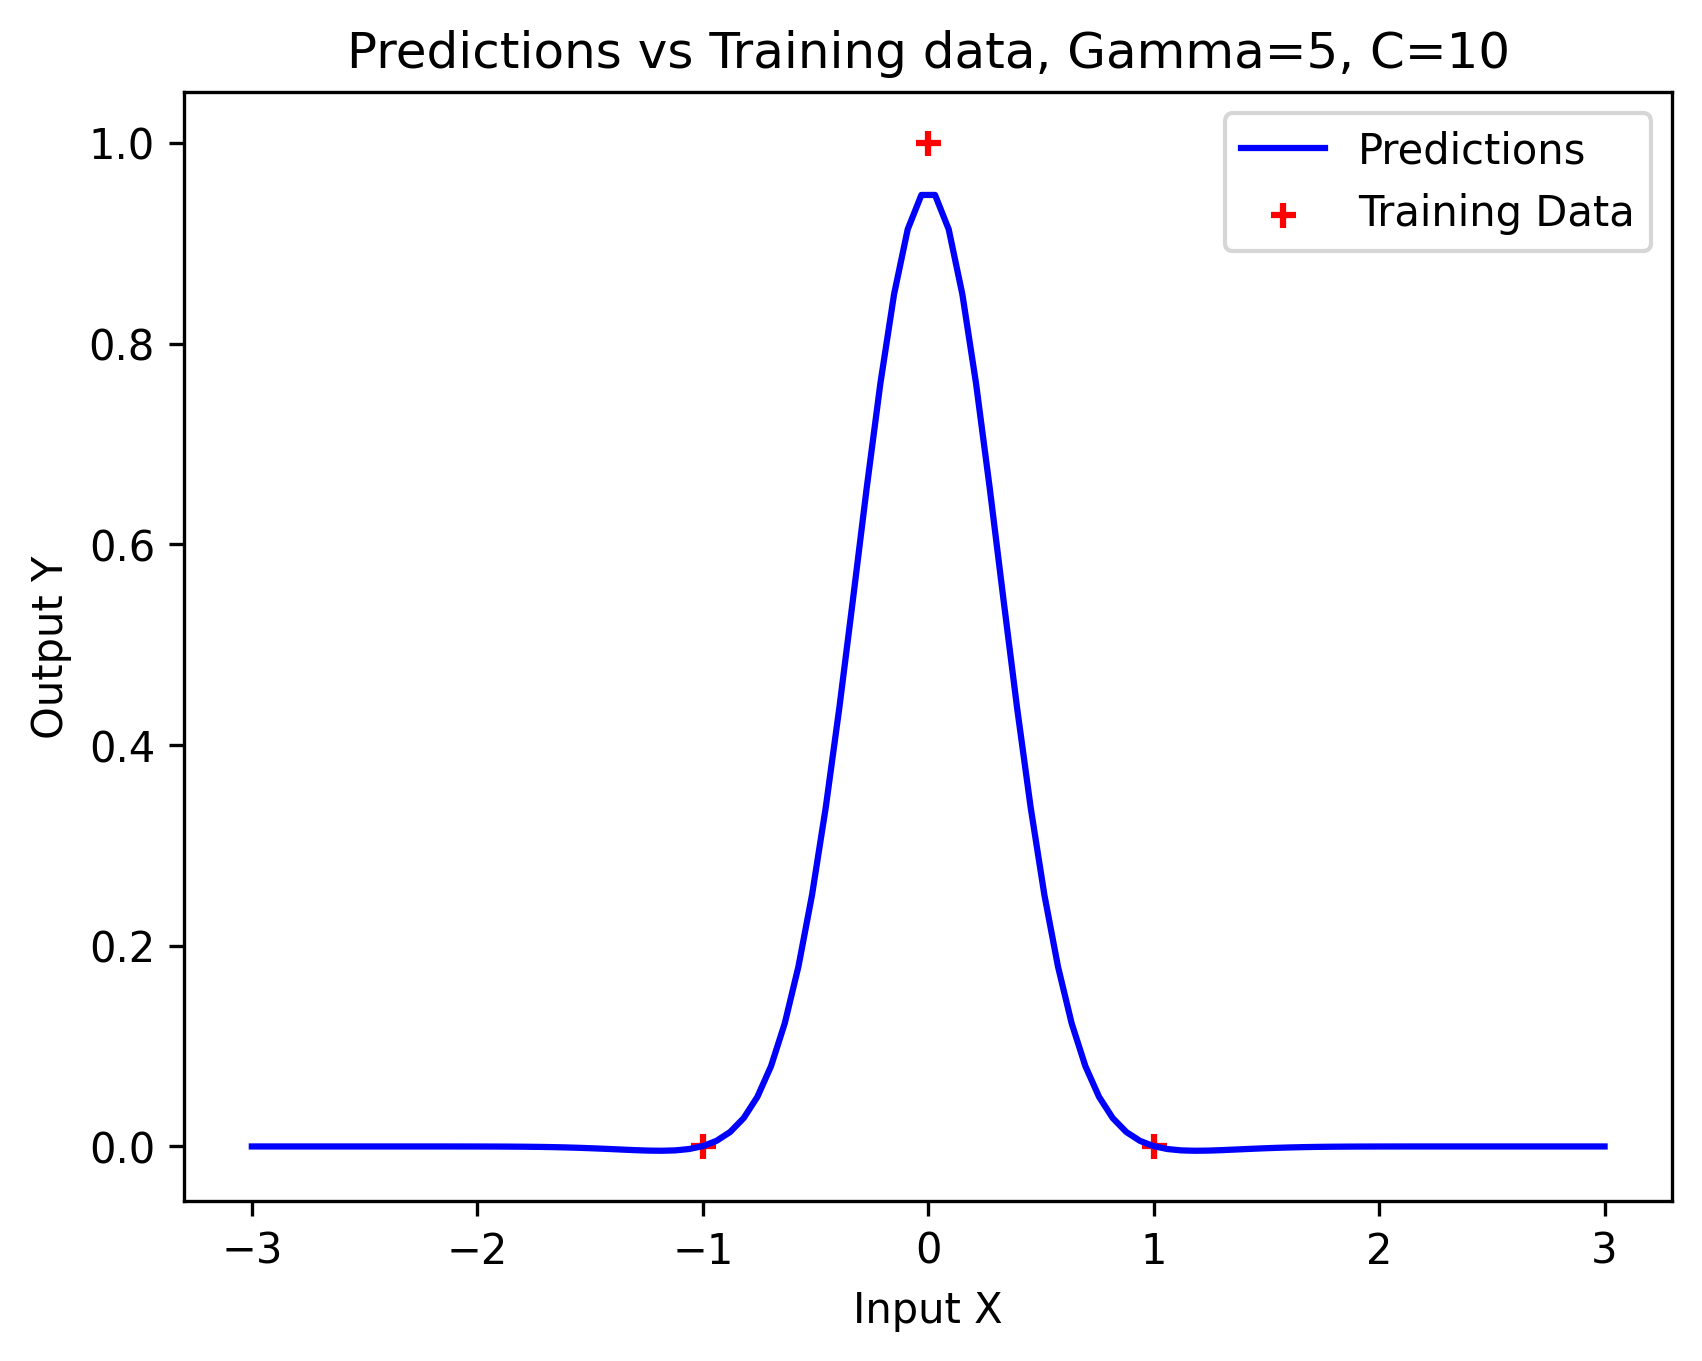
\includegraphics[width=8cm]{kr22.png}}}
\qquad
\subfloat[Gamma = 10, C= 10]{{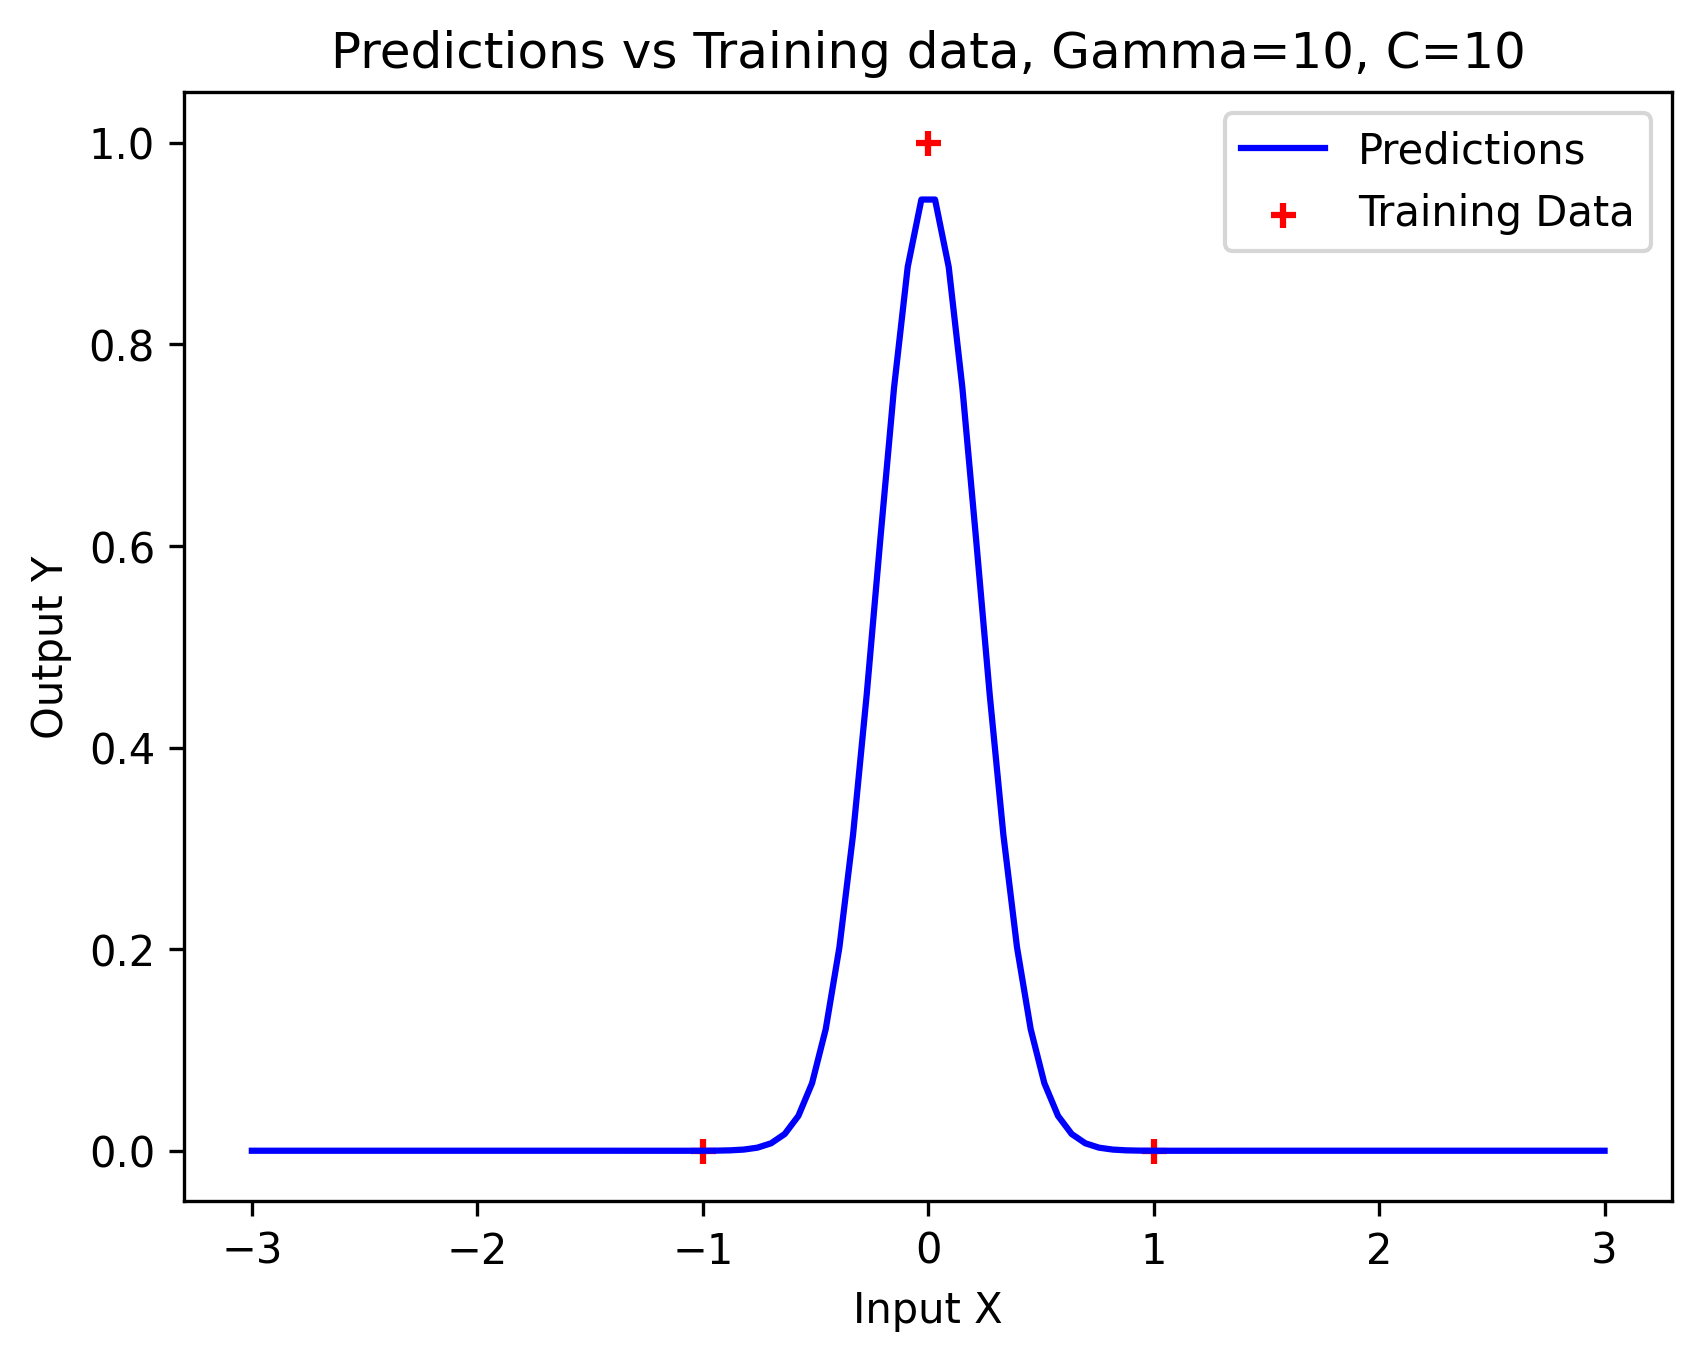
\includegraphics[width=8cm]{kr23.png}}}
\qquad
\subfloat[Gamma = 25, C= 10]{{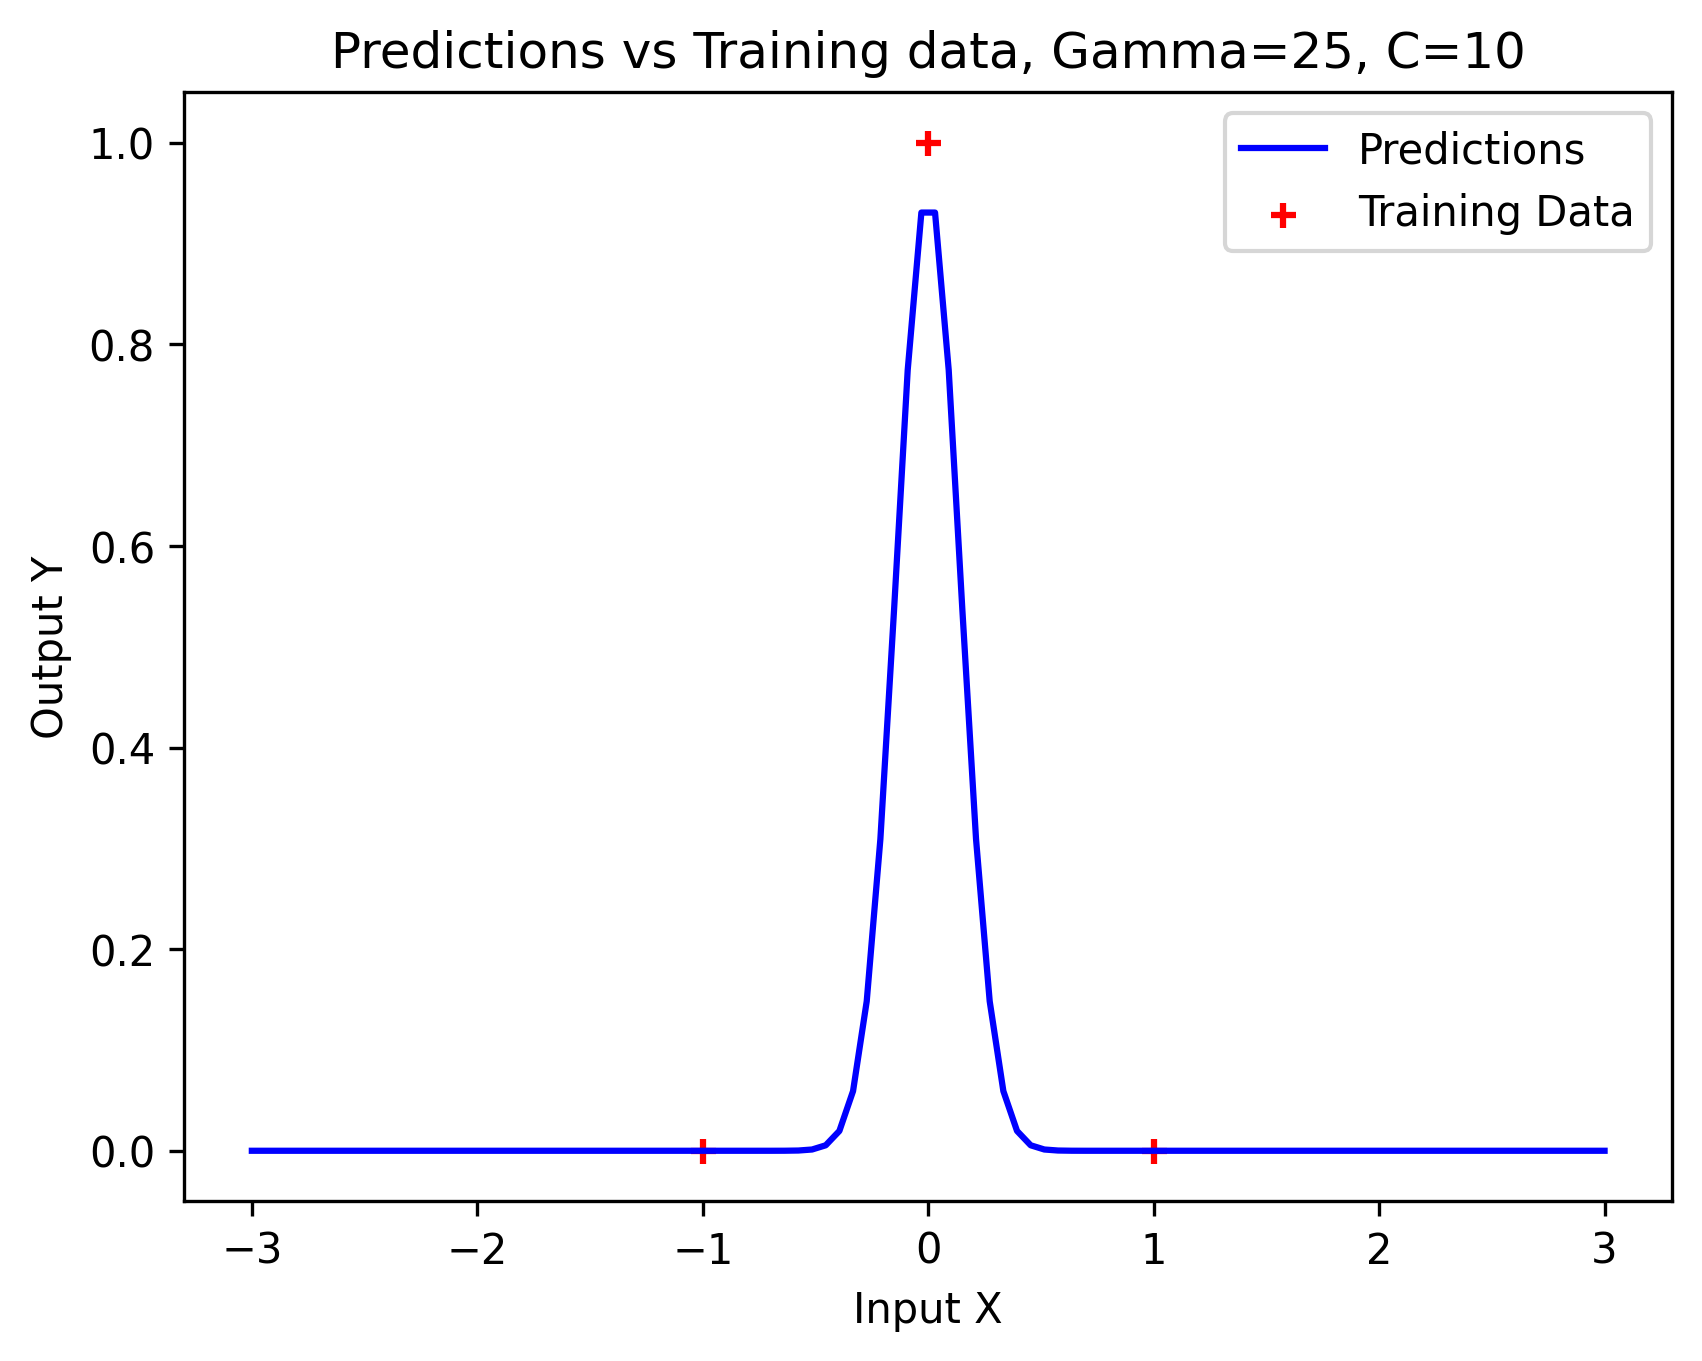
\includegraphics[width=8cm]{kr24.png}}}
\end{figure}
\(\theta_0= -6.5574, \theta_1= 13.4426 , \theta_2= -6.5574\)\\
\(\theta_0= -0.4323, \theta_1= 1.2553 , \theta_2= -0.4323\)\\
\(\theta_0= -0.0061, \theta_1= 0.9525 , \theta_2= -0.0061\)\\
\(\theta_0= -0.0, \theta_1= 0.9524 , \theta_2= -0.0\)\\
\(\theta_0= -0.0, \theta_1= 0.9524 , \theta_2= -0.0\)\\

\begin{figure}[h]
\centering
\subfloat[Gamma = 0, C = 100]{{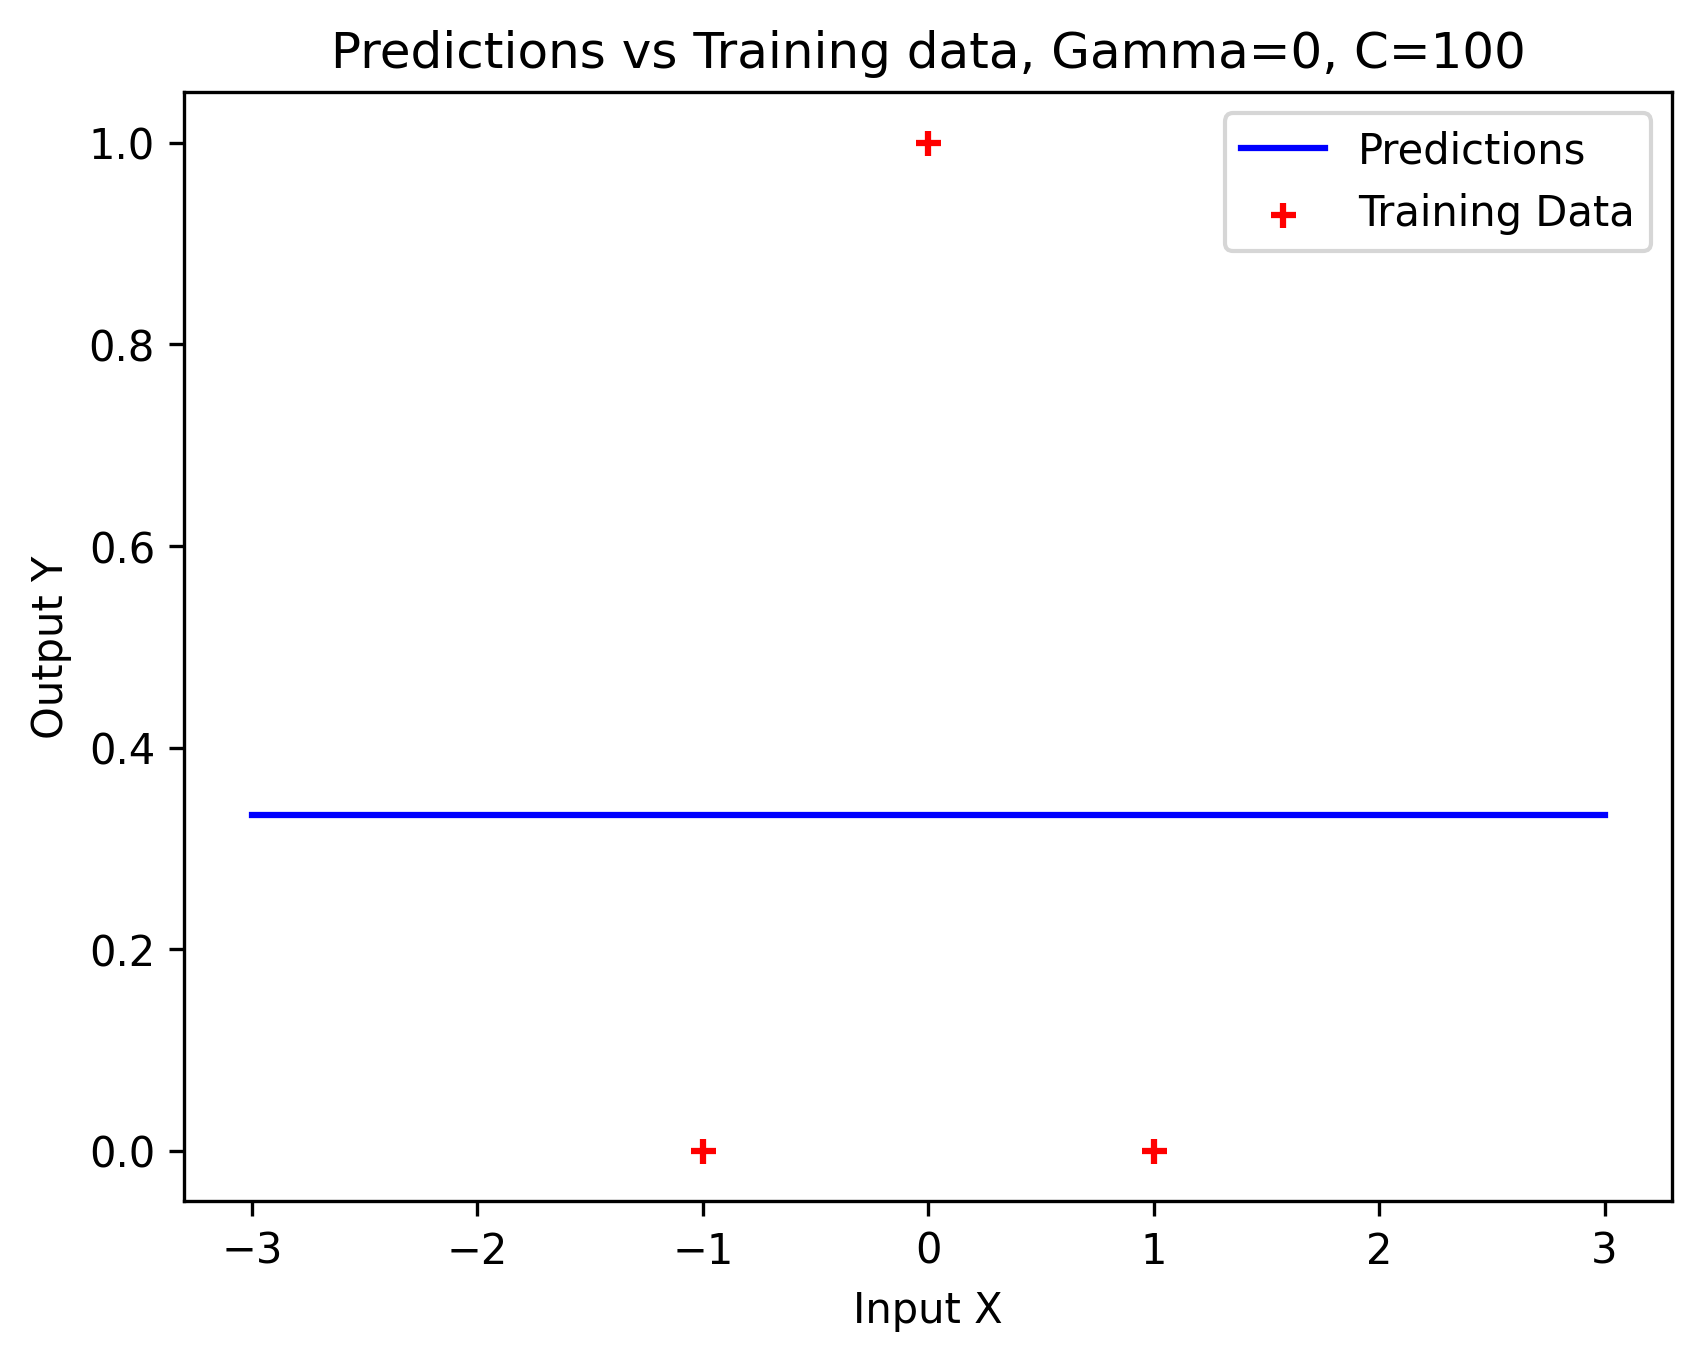
\includegraphics[width=8cm]{kr30.png}}}
\qquad
\subfloat[Gamma = 1, C = 100]{{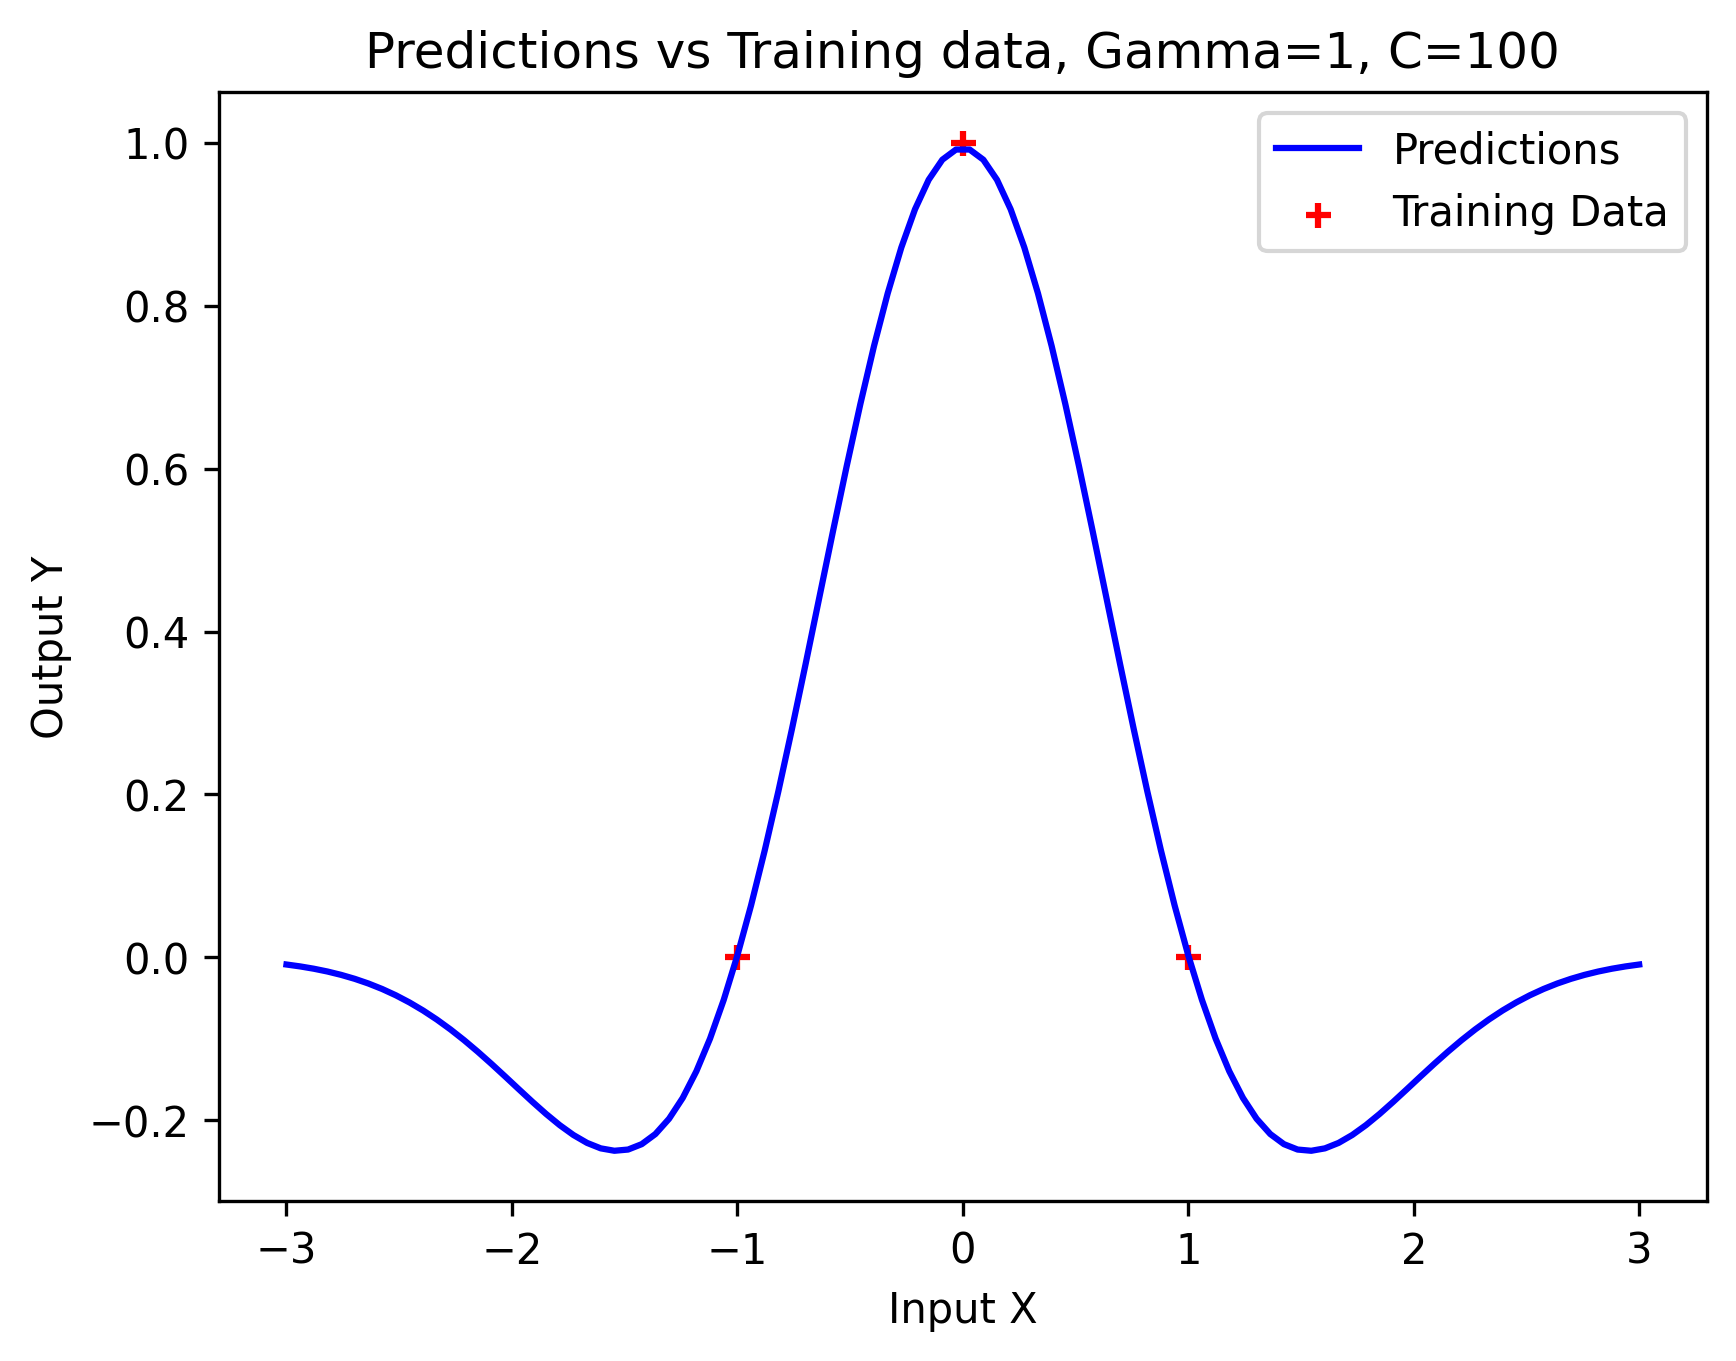
\includegraphics[width=8cm]{kr31.png}}}
\qquad
\subfloat[Gamma = 5, C= 100]{{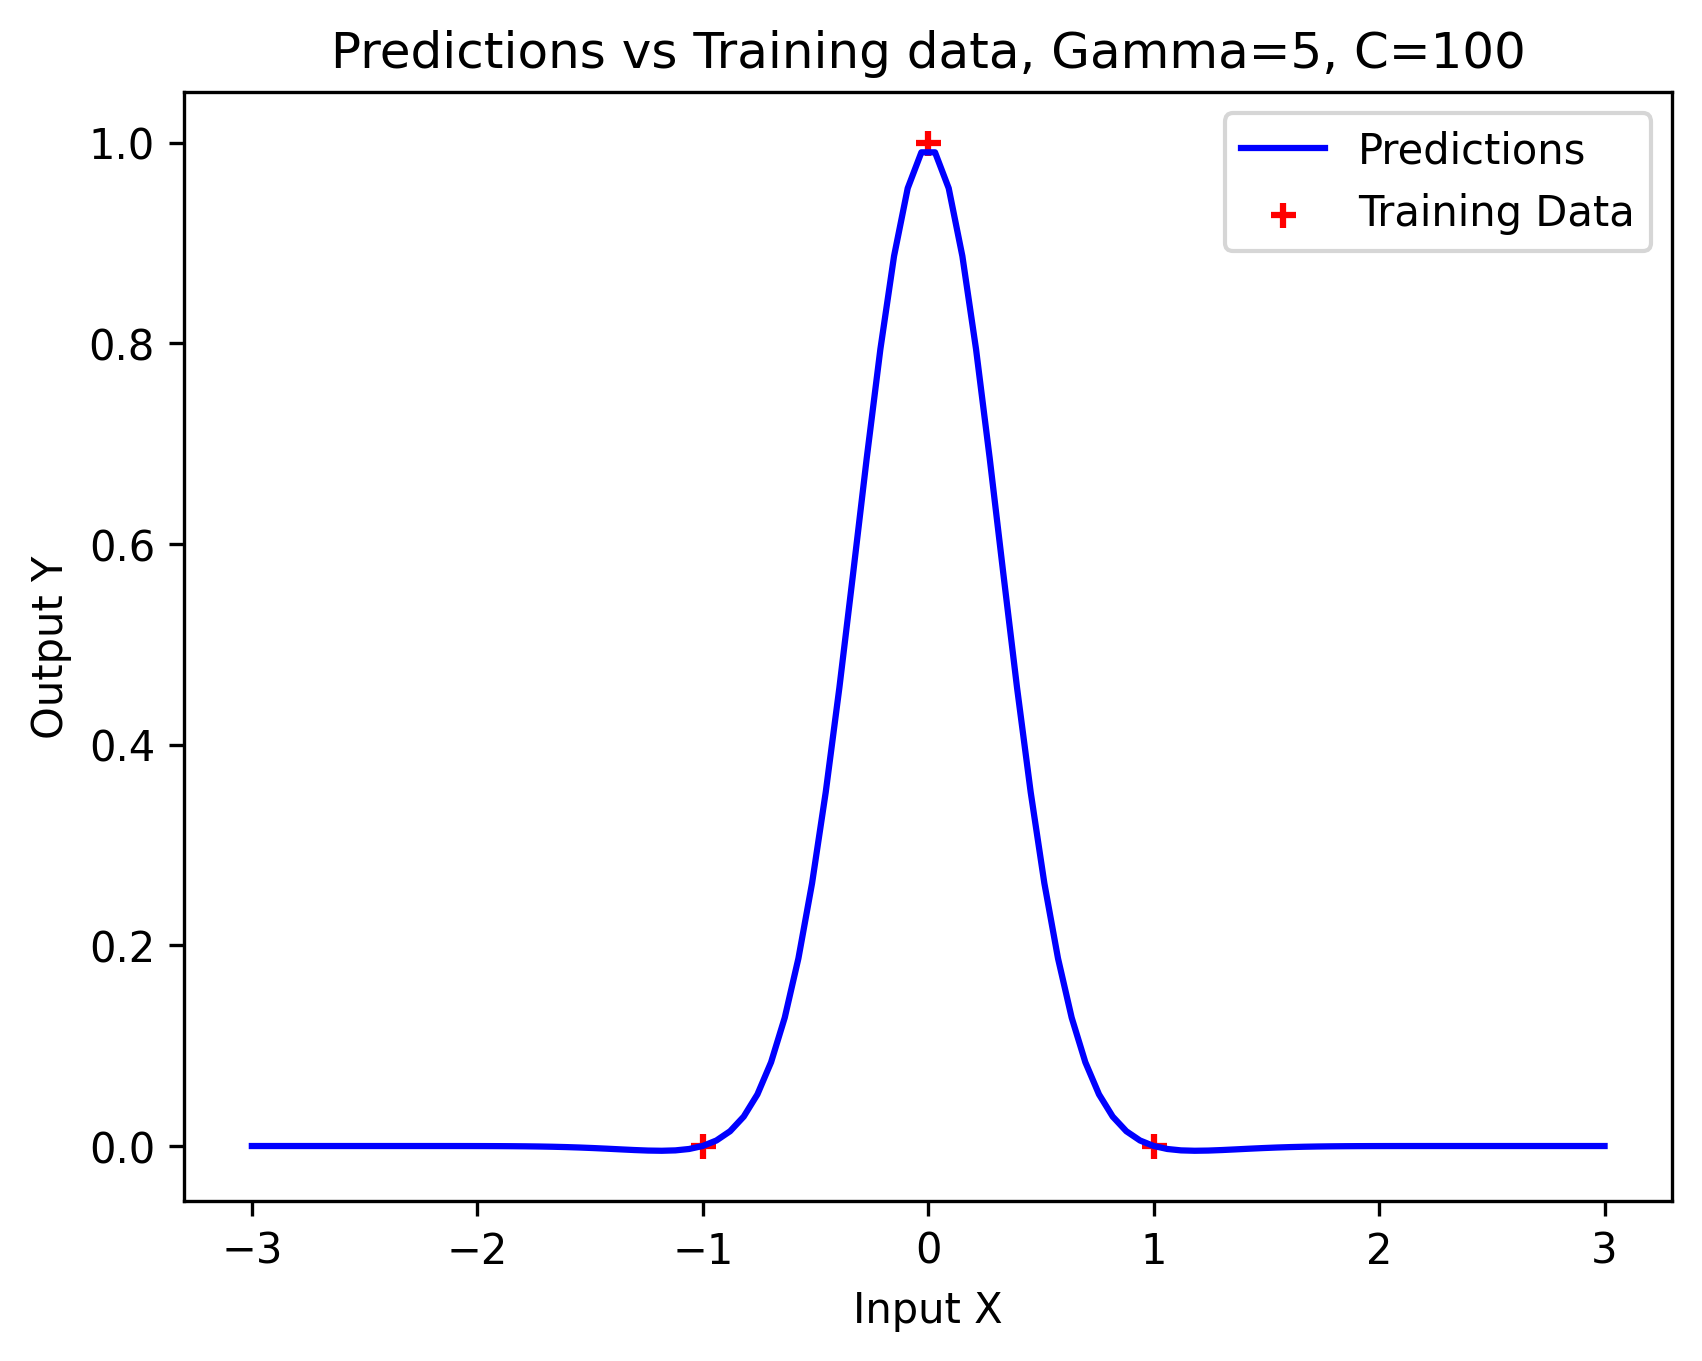
\includegraphics[width=8cm]{kr32.png}}}
\qquad
\subfloat[Gamma = 10, C= 100]{{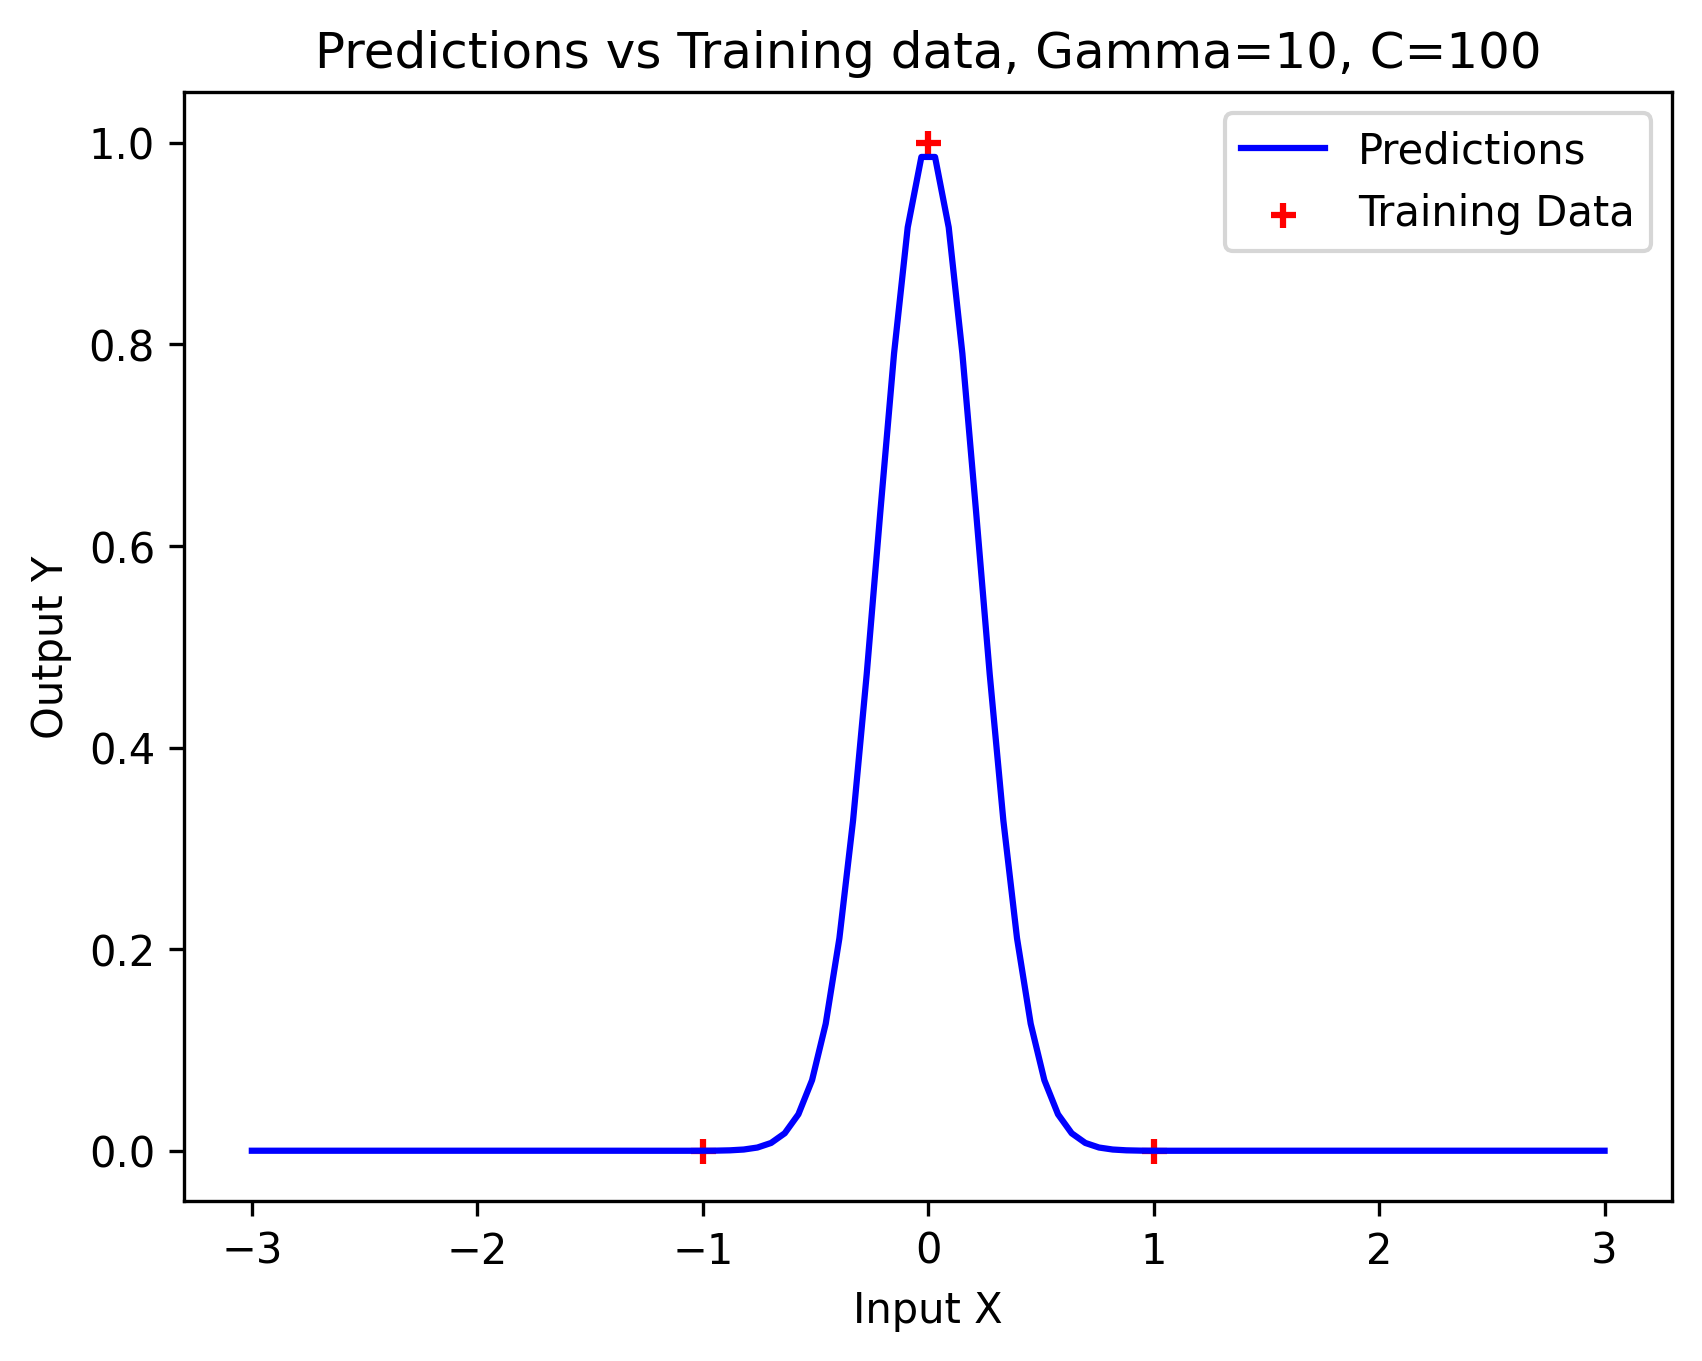
\includegraphics[width=8cm]{kr33.png}}}
\qquad
\subfloat[Gamma = 25, C= 100]{{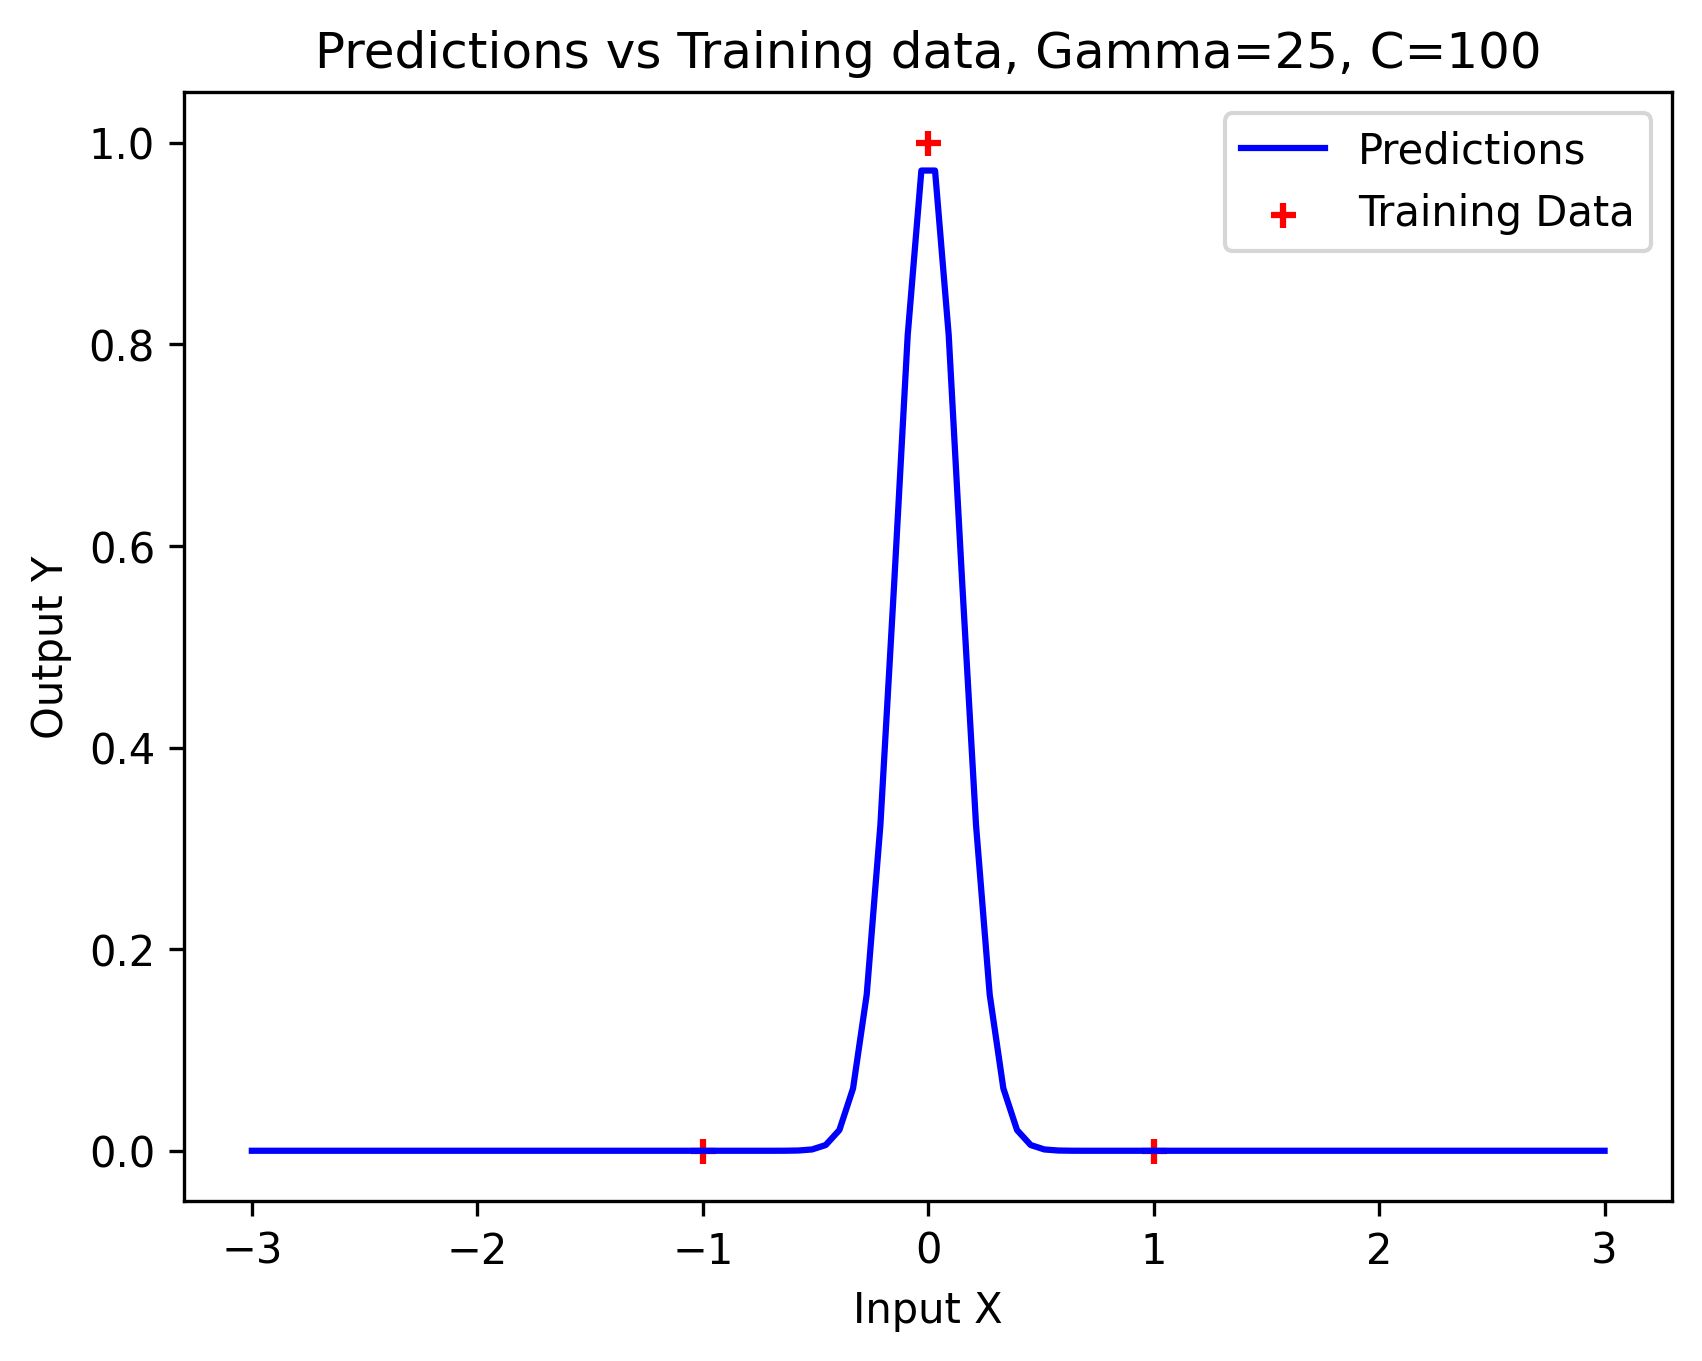
\includegraphics[width=8cm]{kr34.png}}}
\end{figure}
\(\theta_0= -66.5557, \theta_1= 133.4443 , \theta_2= -66.5557\)\\
\(\theta_0= -0.4855, \theta_1= 1.3504 , \theta_2= -0.4855\)\\
\(\theta_0= -0.0067, \theta_1= 0.9951 , \theta_2= -0.0067\)\\
\(\theta_0= -0.0, \theta_1= 0.995 , \theta_2= -0.0\)\\
\(\theta_0= -0.0, \theta_1= 0.995 , \theta_2= -0.0\)\\

\begin{figure}[h]
\centering
\subfloat[Gamma = 0, C = 1000]{{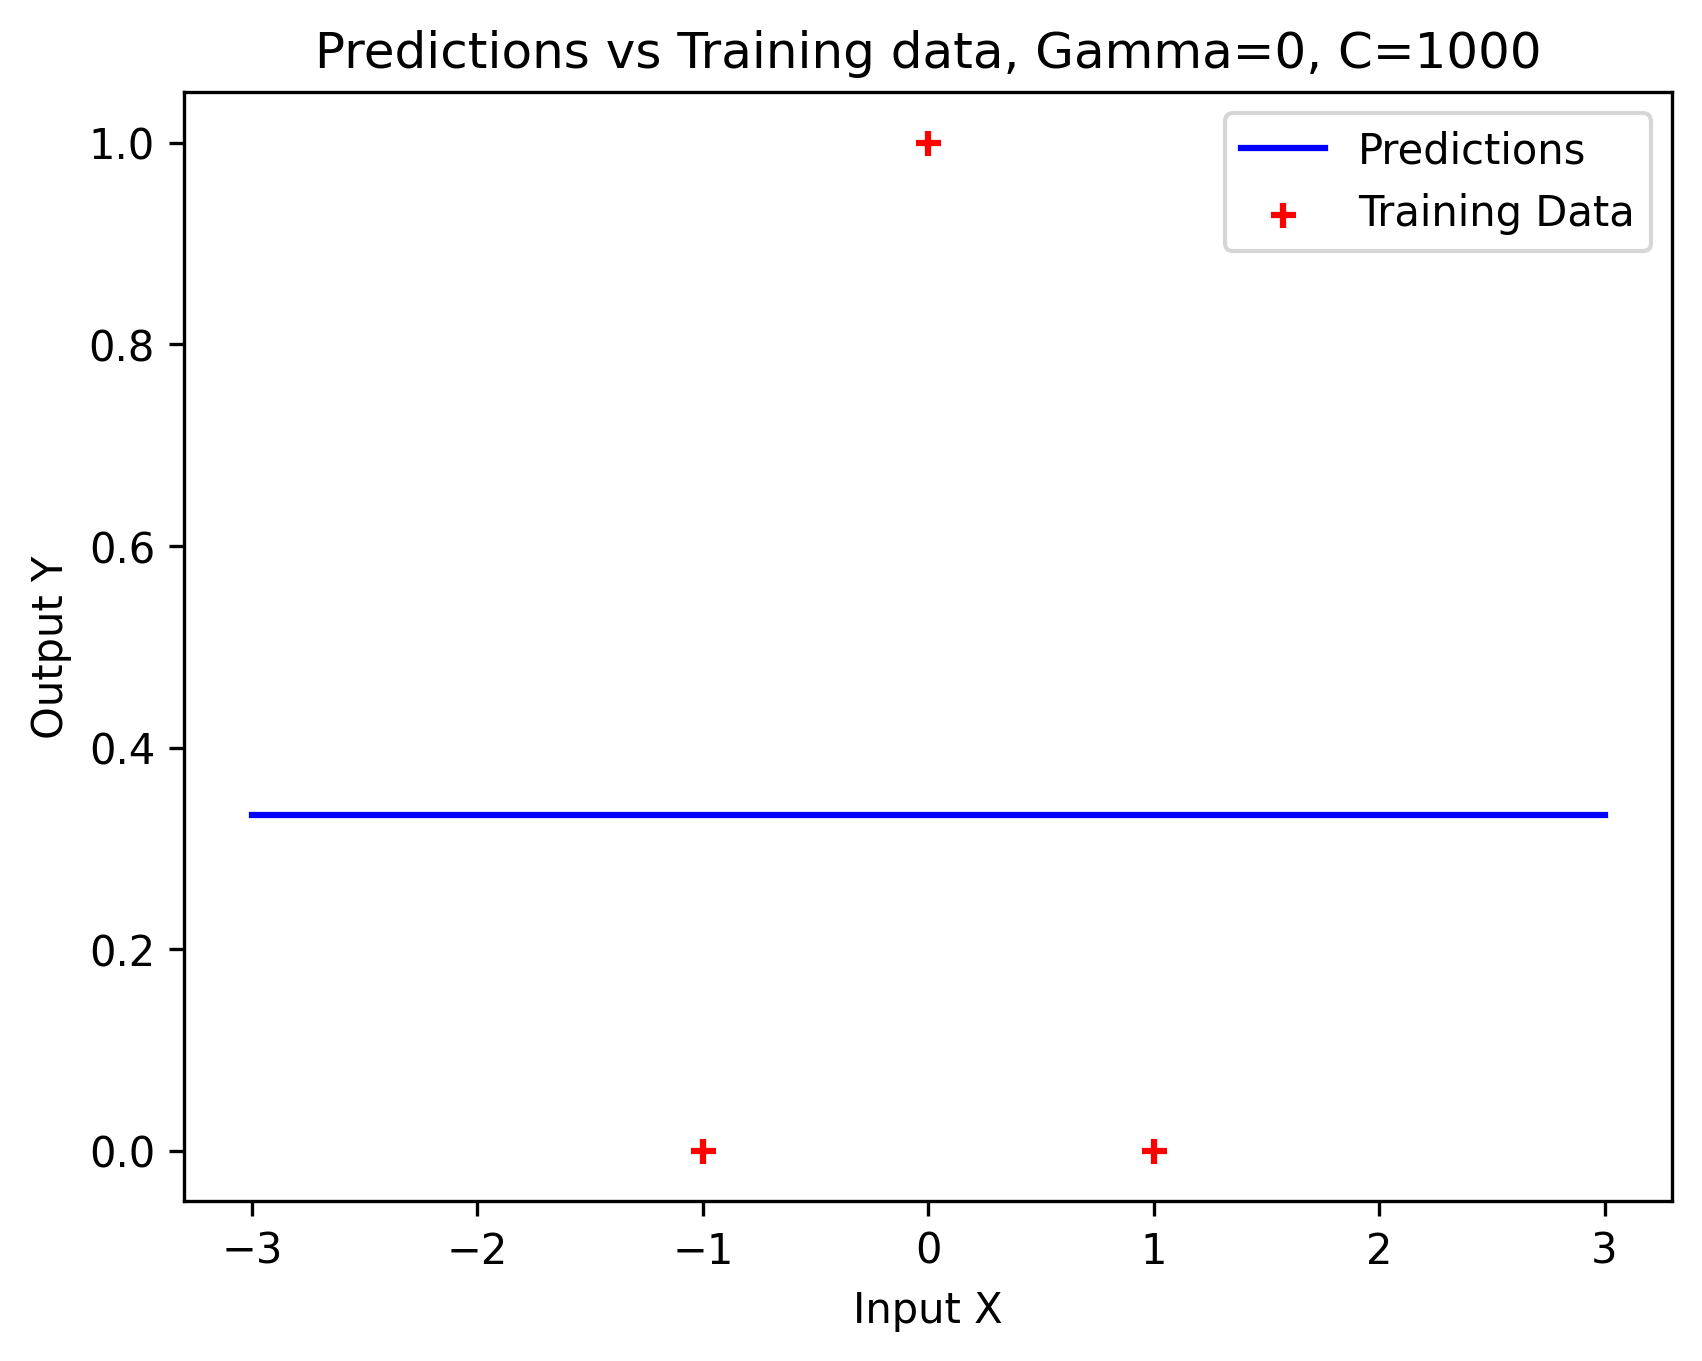
\includegraphics[width=8cm]{kr40.png}}}
\qquad
\subfloat[Gamma = 1, C = 1000]{{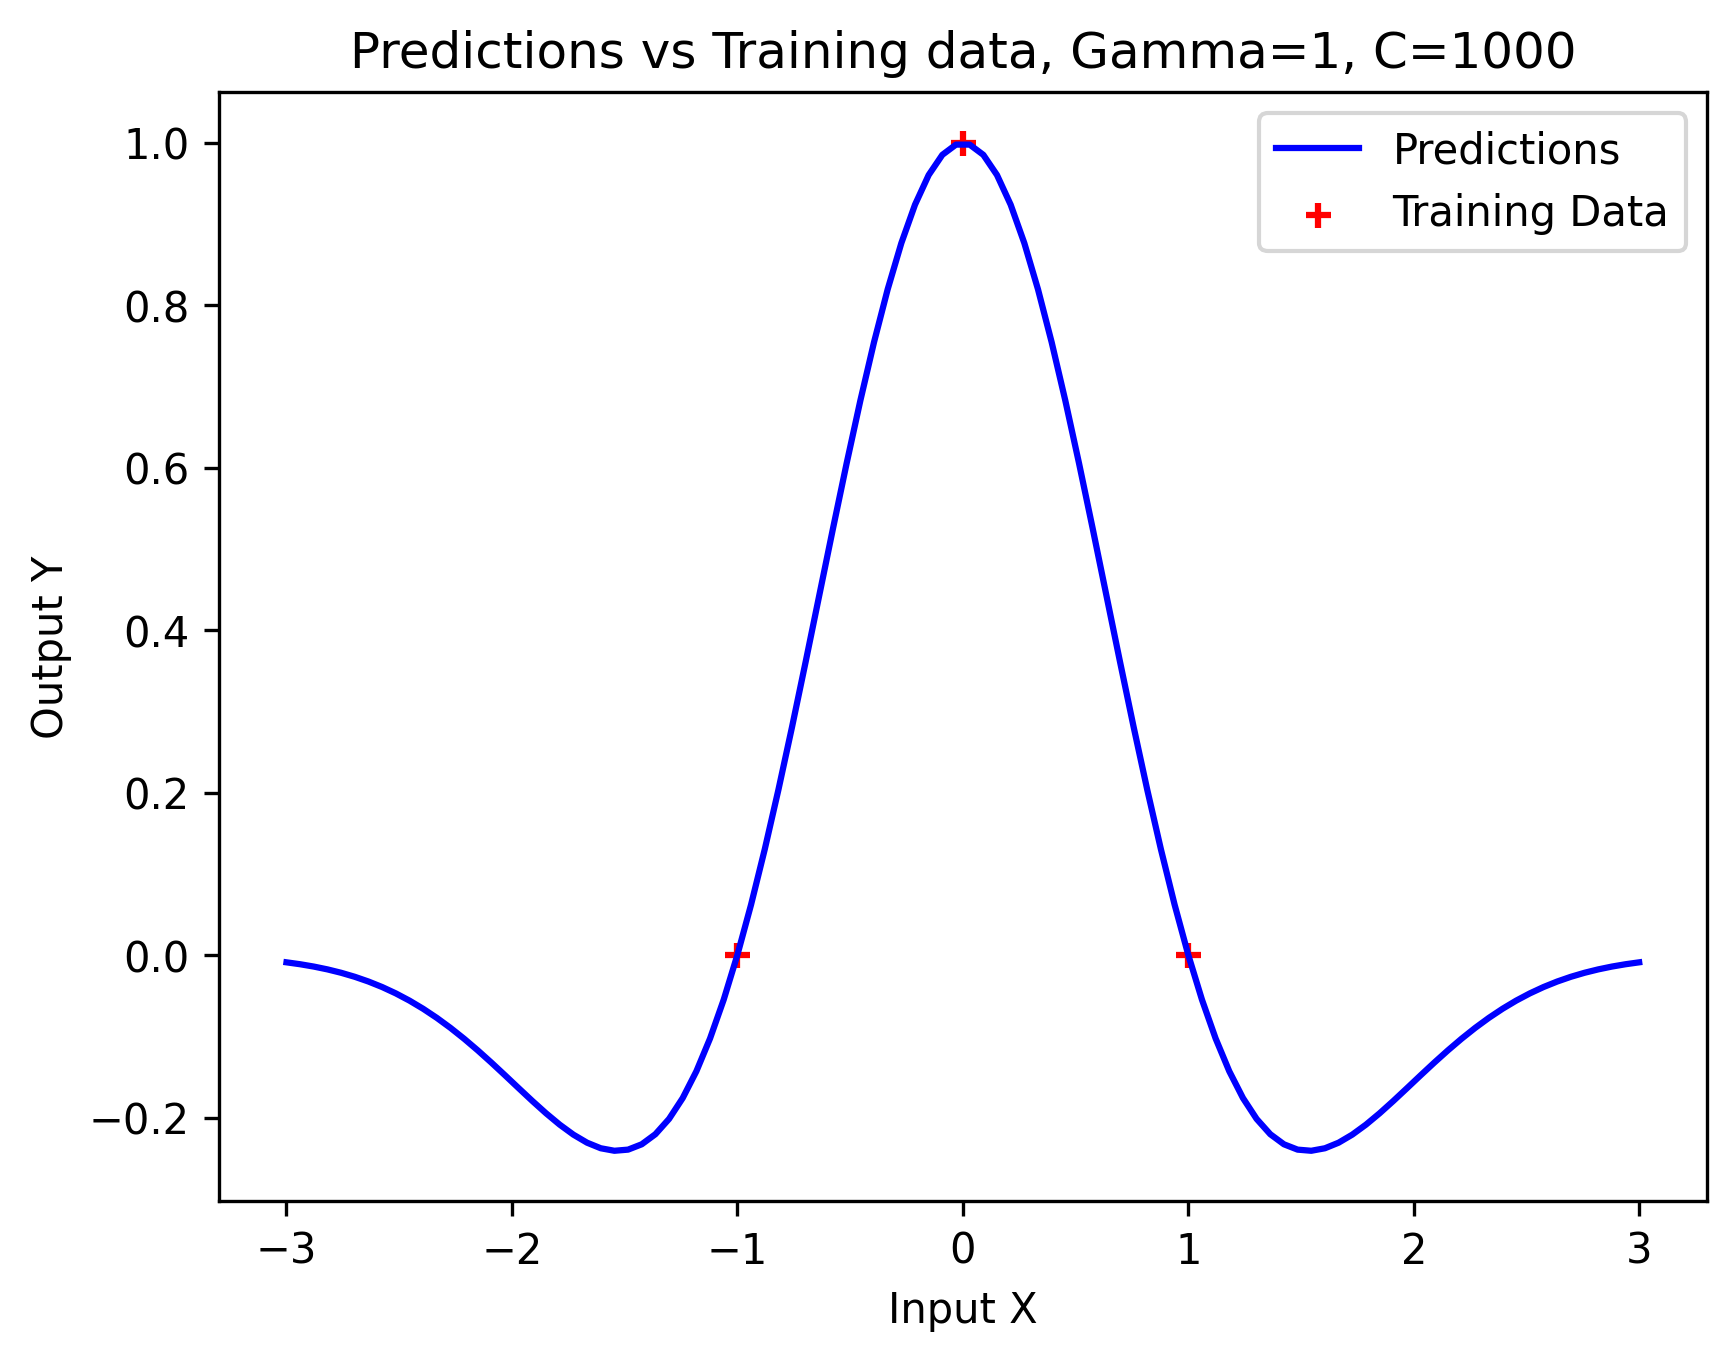
\includegraphics[width=8cm]{kr41.png}}}
\qquad
\subfloat[Gamma = 5, C= 1000]{{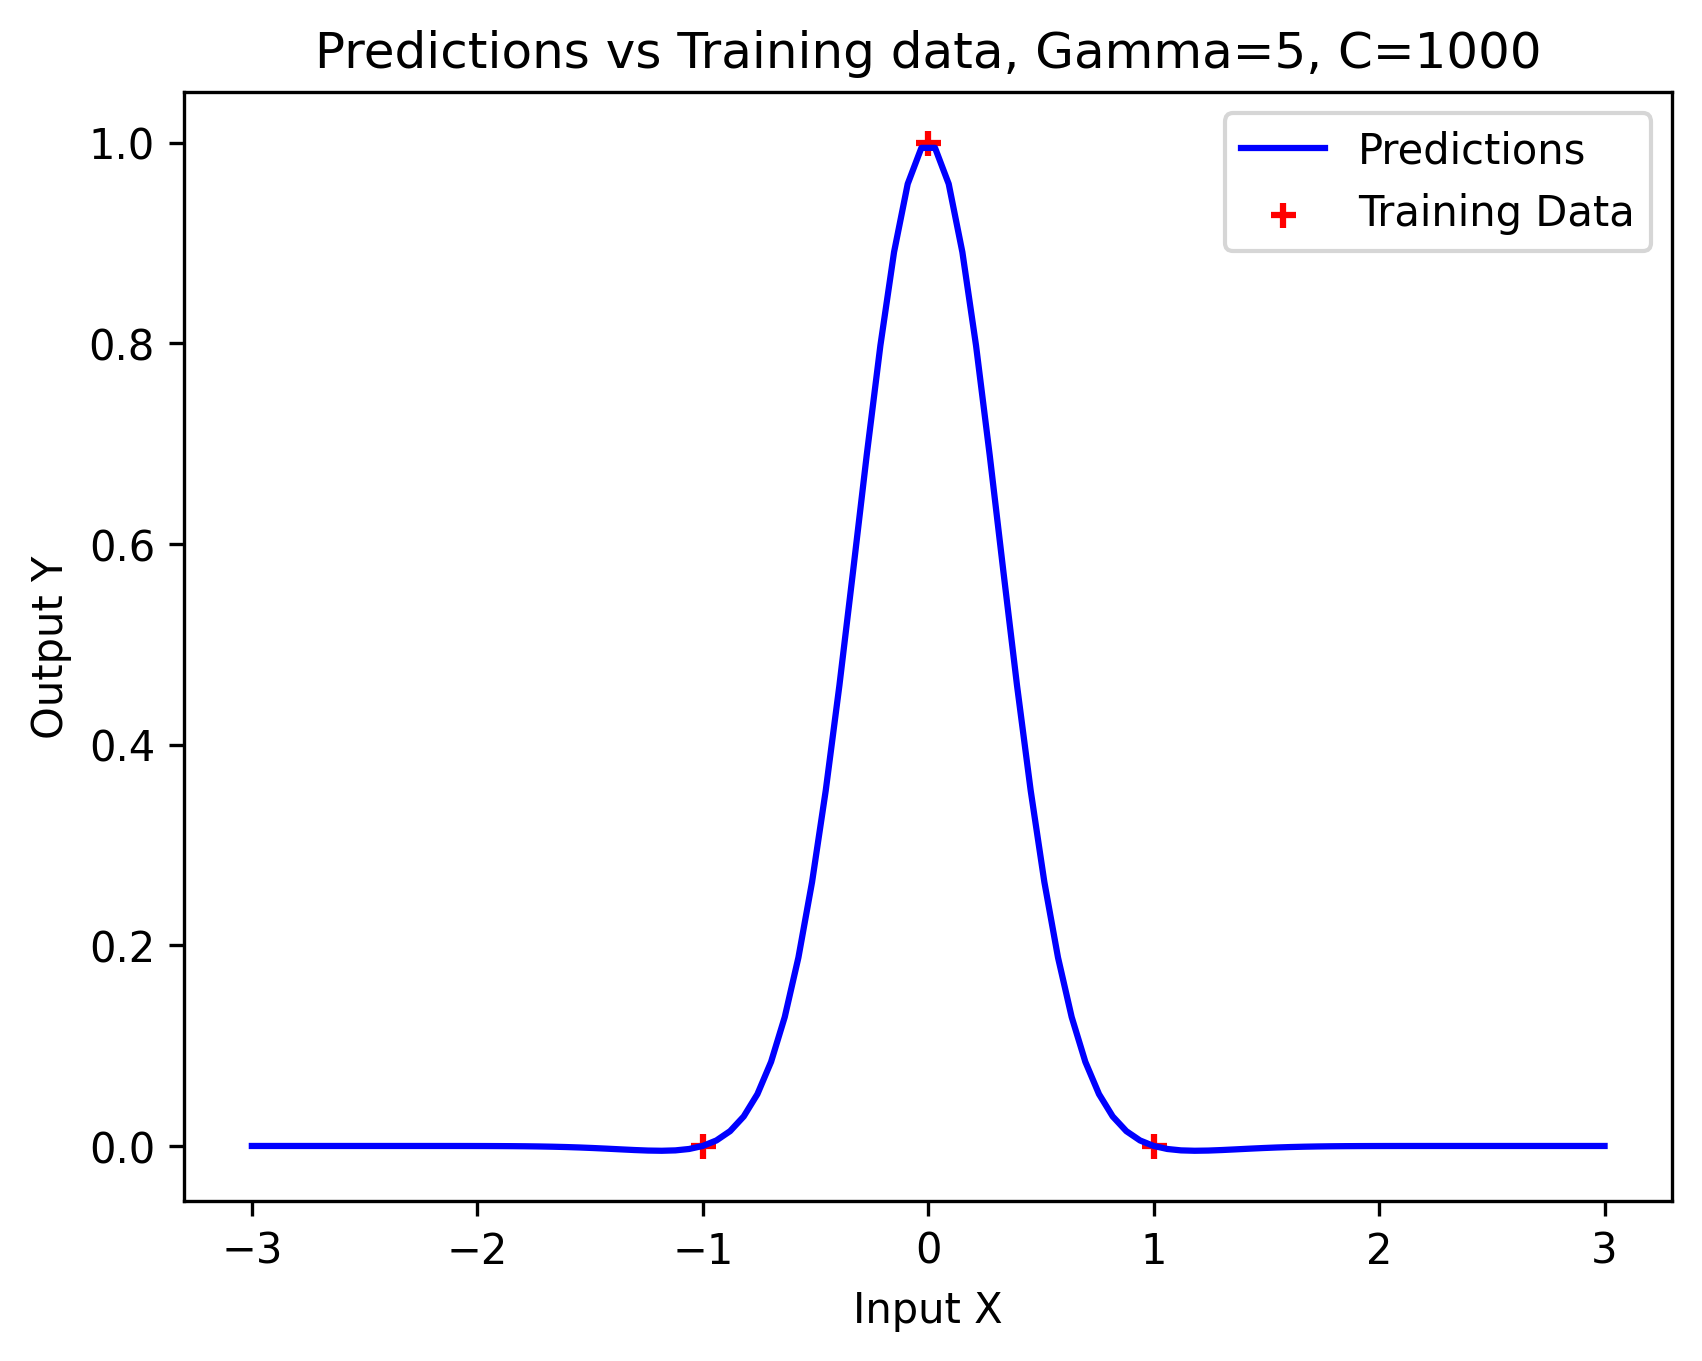
\includegraphics[width=8cm]{kr42.png}}}
\qquad
\subfloat[Gamma = 10, C= 1000]{{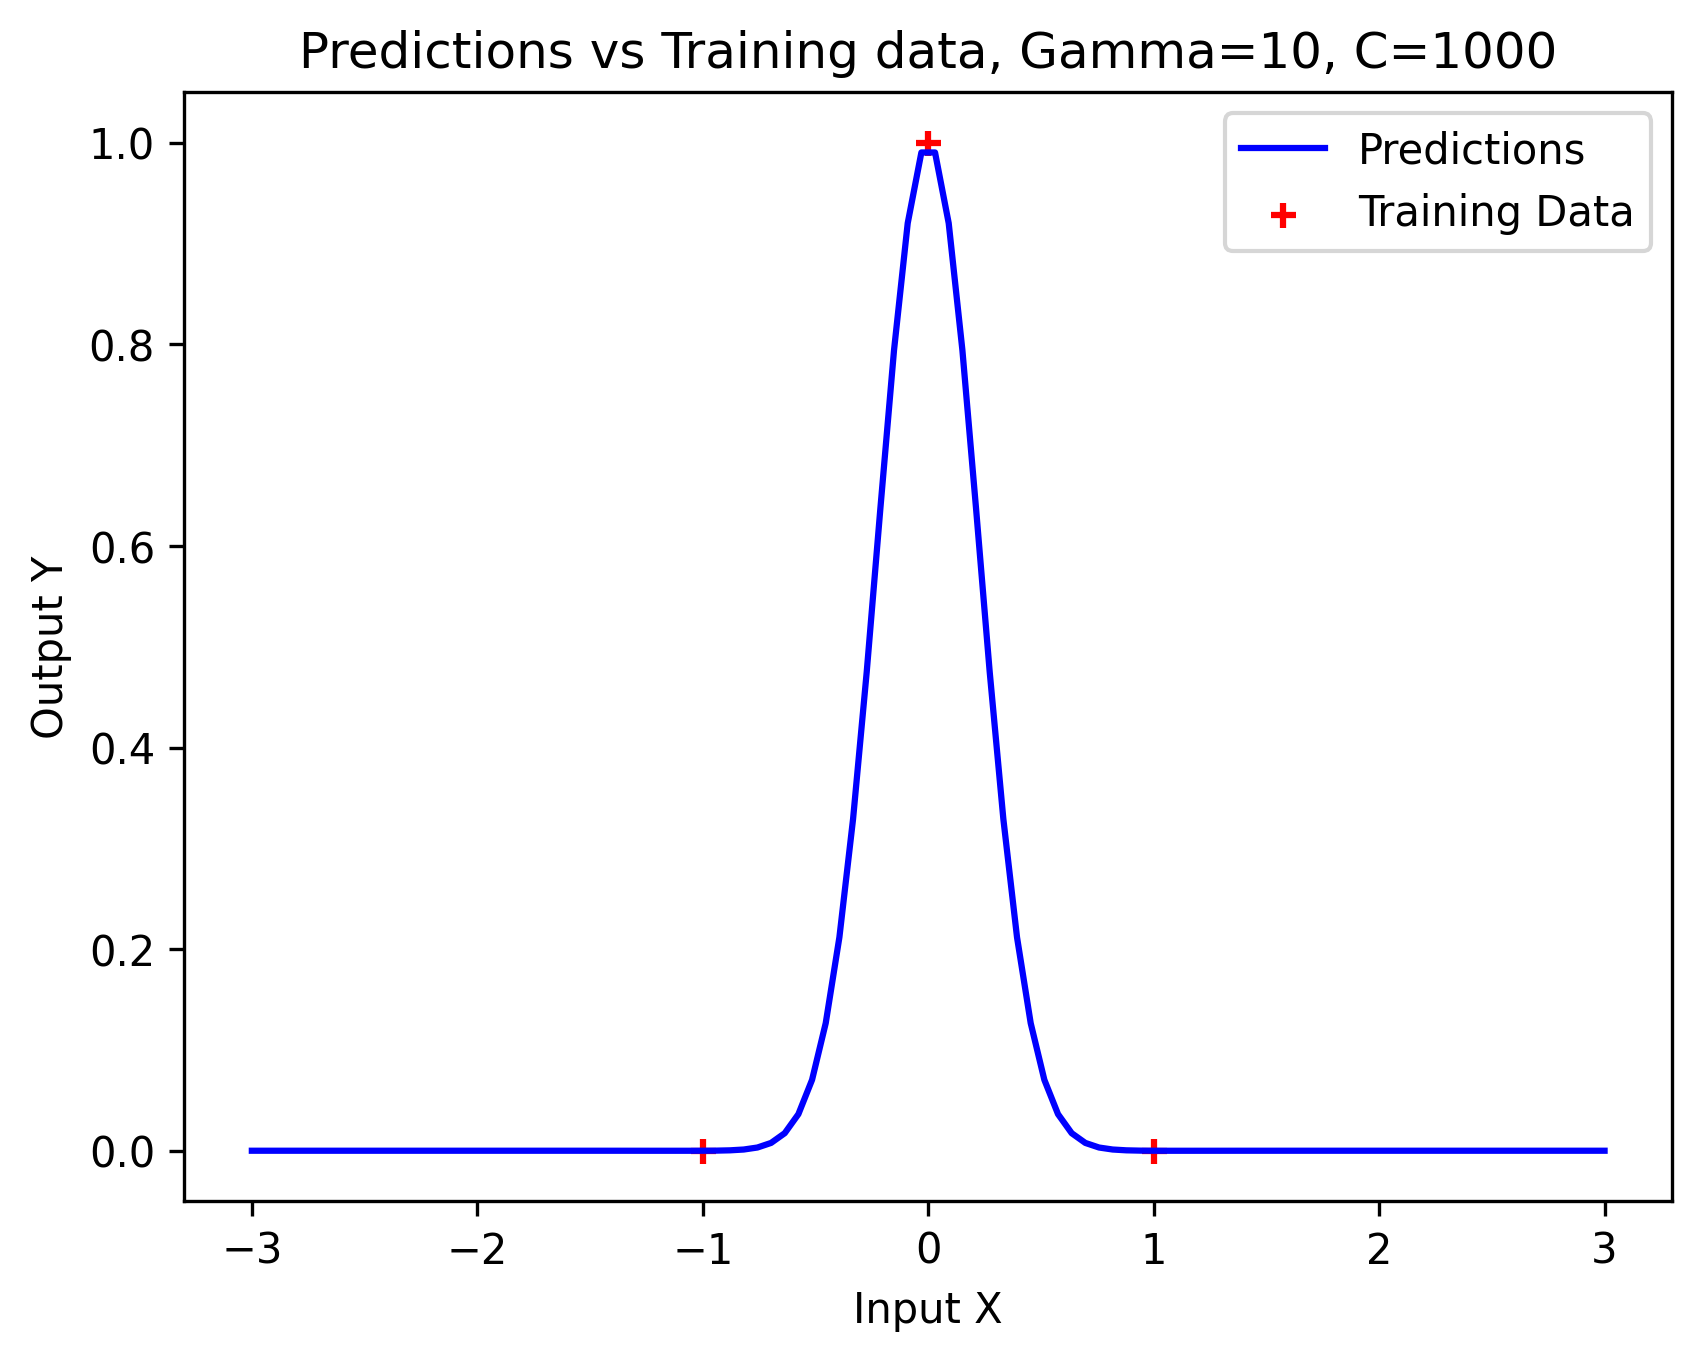
\includegraphics[width=8cm]{kr43.png}}}
\qquad
\subfloat[Gamma = 25, C= 1000]{{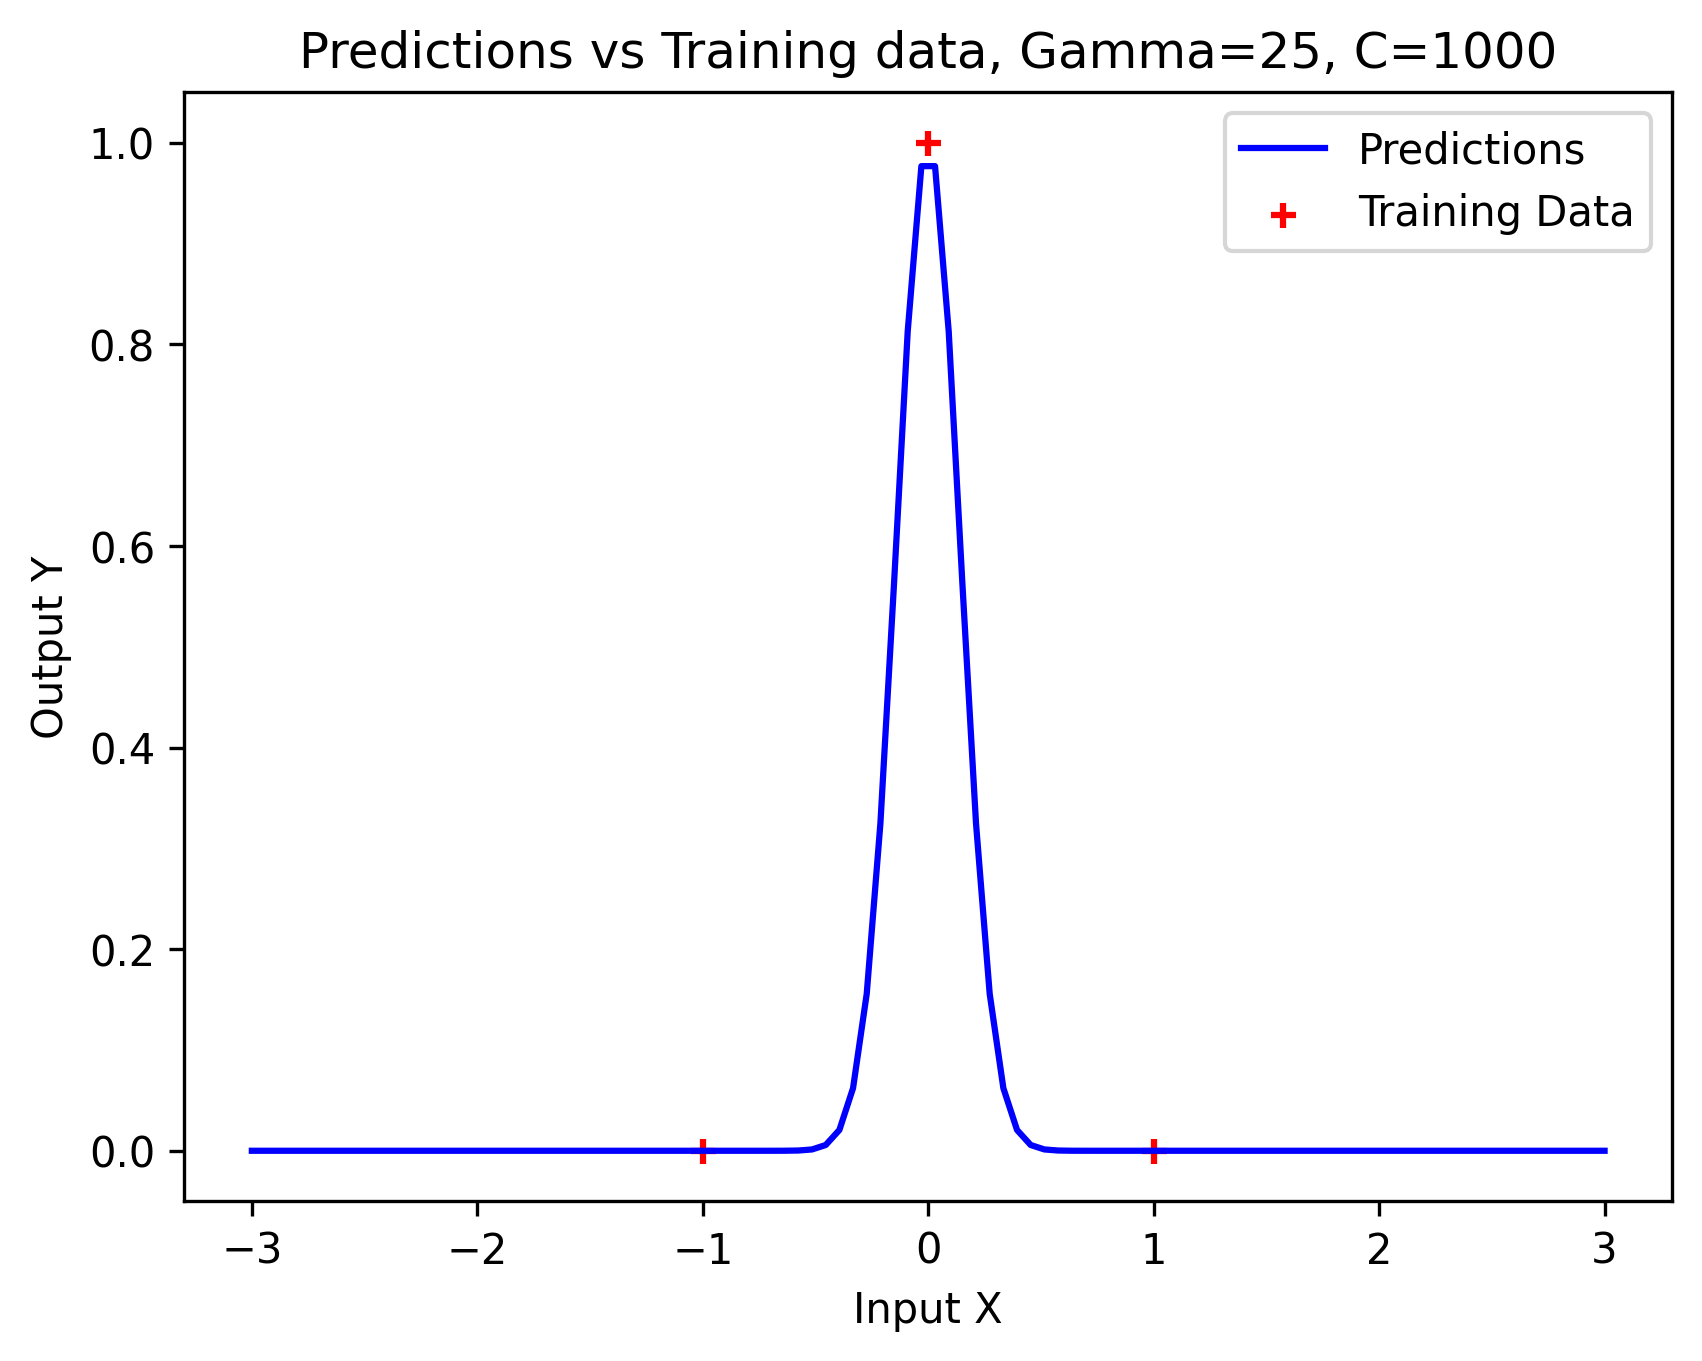
\includegraphics[width=8cm]{kr44.png}}}
\end{figure}
\(\theta_0= -666.5556, \theta_1= 1333.4444 , \theta_2= -666.5556\)\\
\(\theta_0= -0.4914, \theta_1= 1.3609 , \theta_2= -0.4914\)\\
\(\theta_0= -0.0067, \theta_1= 0.9996 , \theta_2= -0.0067\)\\
\(\theta_0= -0.0, \theta_1= 0.9995 , \theta_2= -0.0\)\\
\(\theta_0= -0.0, \theta_1= 0.9995 , \theta_2= -0.0\)\\

\clearpage
\subsection{D}
Kernalised Ridge Regression works by applying a L2 penalty to normal linear regression to shrink parameters down to near 0 that aren't as important to the model in an effort to prevent overfitting. This used along side a kernel can introduce non-linearity to the regressor by introducing new features that are non-linear depending on the type of kernel used. In this case we use a Gaussian kernel to introduce new features hence enabling us to fit a non-linear curve to our data. When we vary our values of C and Gamma, we alter how much of a penalty does the L2 penalty give and also alter how much each of our new features introduced by our kernel effects the slope of our curve. From our data we can see that lower values of Gamma give us much more curved predictions while higher values of gamma snap to the data points. Lower values of C allow for much more of our data to be underfitted while higher values of C do not. When we take these 2 together, Gamma gives us the slope of our line due to introducing non-linear features while C reigns in the slope by giving a penalty to parameters that are not as important in dictating the slope of our line. We can see this in our data, as our value of Gamma is increasing, C gives a more strict penalty hence why more of out parameters are approaching 0(I've rounded the data).  In terms of behaviour between KNN and Kernalised Ridge Regression, Kernalised Ridge Regression allows for more flexible models overall as we can tune both C and Gamma, whiles in KNN we can only tune Gamma. This leads to better predictions as we can get more general and flexible models. KNN seems to much more readily snap to data and give a range of data the same Y output whilst for the same value of Gamma in KRR, it's more general. 

\end{document}
